\thispagestyle{thachthuctoanhocnone}
\pagestyle{thachthuctoanhoc}
\everymath{\color{thachthuctoanhoc}}
\graphicspath{{../thachthuctoanhoc/pic/}}
\begingroup
\AddToShipoutPicture*{\put(0,616){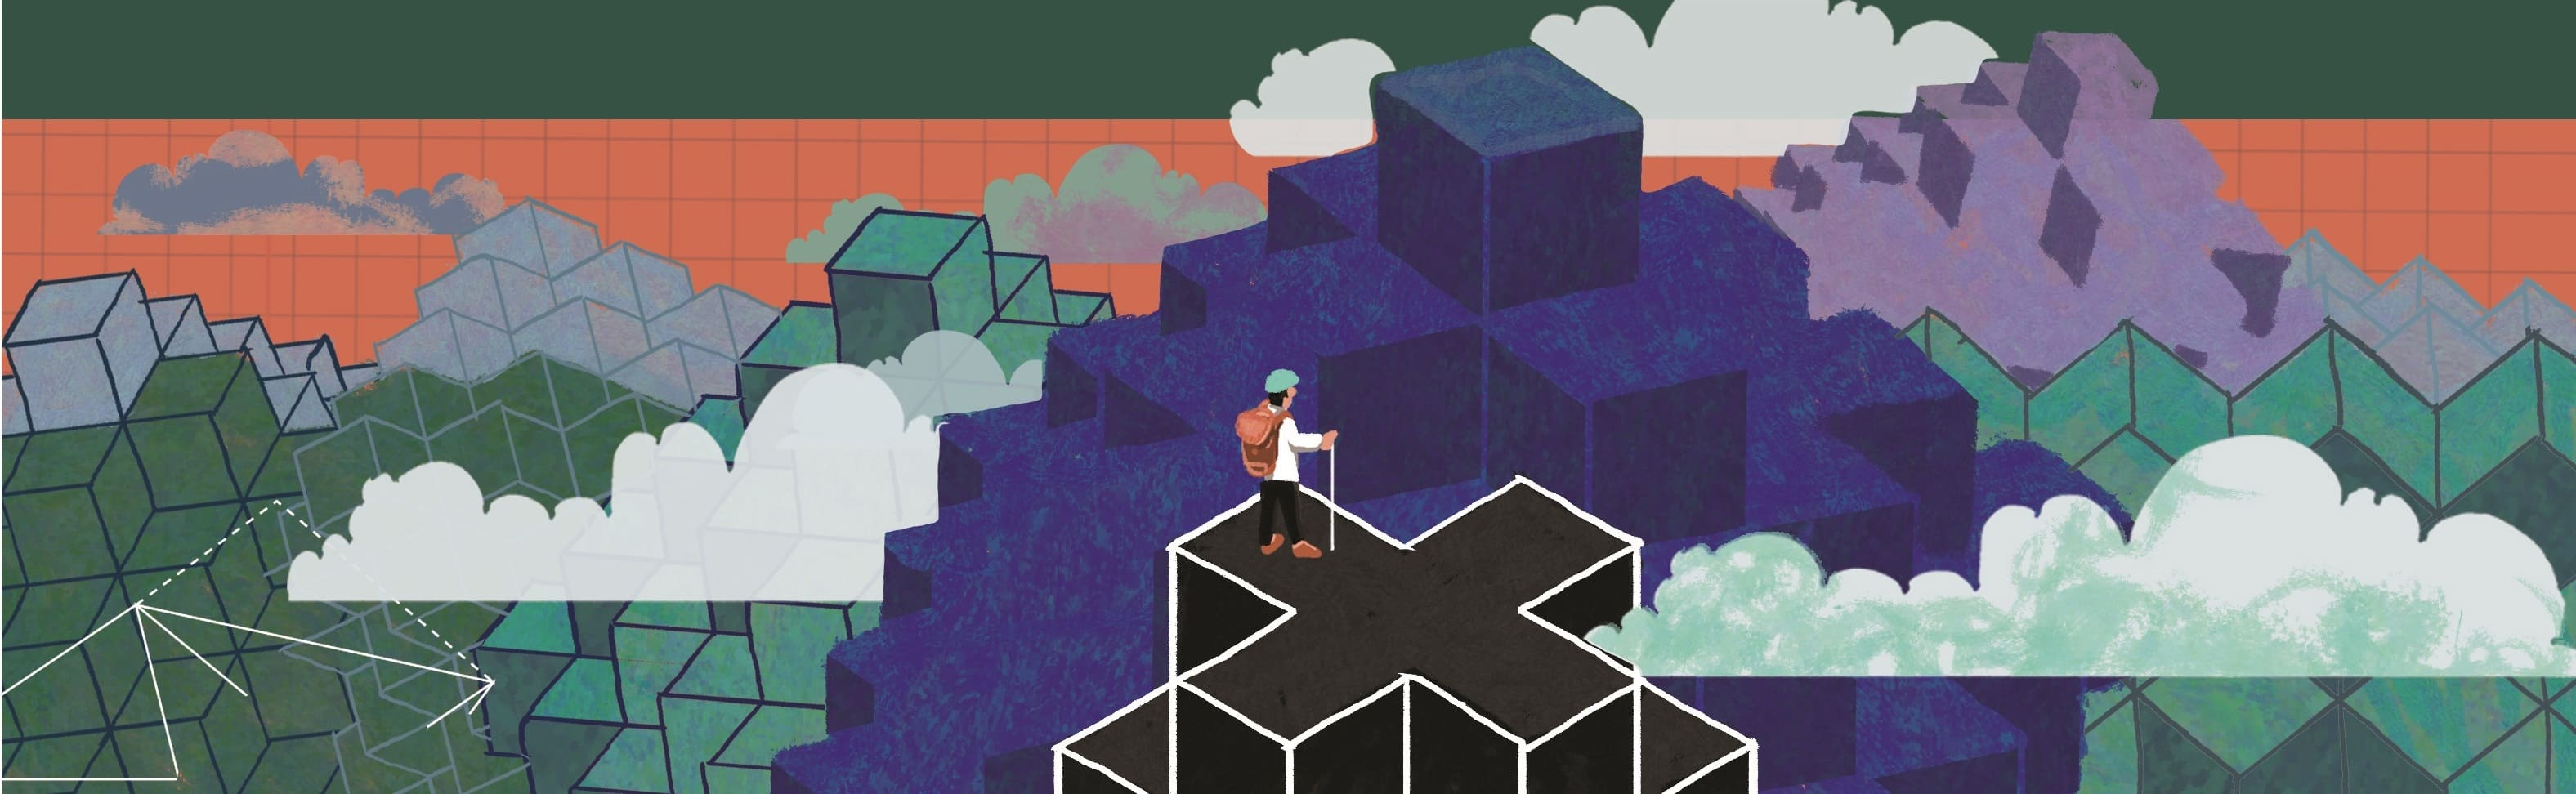
\includegraphics[width=19.3cm]{../thachthuctoanhoc/bannerthachthuc}}}
\centering
\vspace*{4cm}
\endgroup
\vspace*{-8pt}
\begin{tBox}
	\begin{itemize}[leftmargin = 13pt, itemsep = 1.0pt] 
		\item Mỗi bài toán đề xuất (kèm theo lời giải) cần được nêu rõ là bài sáng tác hay bài sưu tầm.
%		\item Mỗi bài toán đề xuất (kèm theo lời giải) cần được nêu rõ là bài sáng tác hay bài sưu tầm (nếu là bài sưu tầm, cần ghi rõ nguồn).
		\item Bài giải cho mỗi bài toán cần được trình bày trong một file riêng hoặc
		một tờ giấy riêng.
		\item  Người đề xuất bài toán hoặc gửi bài giải cho các bài toán trong mục ``Thách thức kỳ này" cần ghi rõ họ, đệm, tên và nơi làm việc/học tập, số điện thoại liên hệ. Nếu là học sinh (hoặc sinh viên) cần ghi rõ là học sinh lớp mấy (hoặc sinh viên năm thứ mấy).
		\item Các bài toán trong mục Thách thức kỳ này hướng tới các độc giả là học sinh phổ thông; được phân chia thành các mức độ $B$, $A$, và được sắp xếp theo độ khó tăng dần, theo đánh giá chủ quan của Ban biên tập. Các bài toán mức độ $B$ không đòi hỏi các kiến thức vượt quá chương trình môn Toán cấp THCS; các bài toán mức độ $A$ không đòi hỏi các kiến thức vượt quá chương trình môn Toán cấp THPT.
		\item Cách thức gửi bài toán đề xuất hoặc lời giải: gửi file thu được bằng cách scan, ảnh chụp (rõ nét) của bản viết tay, hoặc được soạn thảo bằng các phần mềm Latex, Word tới \url{bbt@pi.edu.vn} hoặc gửi qua đường bưu điện tới Tòa soạn (xem địa chỉ tại bìa $2$).
		\item Hạn gửi lời giải cho các bài toán P$651$--P$660$: trước ngày $15/12/2022$.
	\end{itemize}
\end{tBox}
\begin{center}
	\vspace*{-5pt}
	\textbf{\color{thachthuctoanhoc}\color{thachthuctoanhoc}THÁCH THỨC KỲ NÀY}
	\vspace*{-5pt}
\end{center}
%\begin{multicols}{2}
%	\setlength{\abovedisplayskip}{4pt}
%	\setlength{\belowdisplayskip}{4pt}
%	{\color{thachthuctoanhoc}{\usefont{T5}{qag}{b}{n} P641.}}
%	(Mức $B$) Tại mỗi đỉnh của một đa giác lồi $18$ cạnh ở hình dưới đây, người ta ghi một số, sao cho số được ghi ở mỗi đỉnh bằng tổng hai số được ghi ở hai đỉnh kề với nó.
%	\begin{figure}[H]
%		\vspace*{-5pt}
%		\centering
%		\captionsetup{labelformat= empty, justification=centering}
%		\definecolor{ffvvqq}{rgb}{1,0.3333333333333333,0}
%		\definecolor{qqqqffa}{rgb}{0,0,1}
%		\definecolor{qqzzff}{rgb}{0,0.6,1}
%		\begin{tikzpicture}[line cap=round,line join=round,>=triangle 45,x=1cm,y=1cm,scale=0.4]
%			\draw (1.401115339869085,5.50644760016908136) node[anchor=north west] {$X$};
%			\draw (1.4408759814898973,-0.7306378725360659) node[anchor=north west] {$Y$};
%			\draw (-7.8444170535279,2.5008856260029945) node[anchor=north west] {$S$};
%			\draw [color=qqzzff] (0.0915547437082469,-1.9784020259611625)--(1.3147607160299626,-0.9781184915188108);
%			\draw [color=qqzzff] (1.3147607160299626,-0.9781184915188108)--(2.122081224105652,0.3802016464606015); 
%			\draw [color=qqzzff] (2.122081224105652,0.3802016464606015)--(2.4161414998796458,1.932724932666551); 
%			\draw [color=qqzzff] (2.4161414998796458,1.932724932666551)--(2.1614735342261406,3.4921941459791768);
%			\draw [color=qqzzff] (2.1614735342261406,3.4921941459791768)--(1.38879404230183,4.87051428395859);
%			\draw [color=qqzzff] (1.38879404230183,4.87051428395859)--(0.19129957436757605,5.901439596125702);
%			\draw [color=qqzzff] (0.19129957436757605,5.901439596125702)--(-1.2865743636076452,6.4606252749959765);
%			\draw [color=qqzzff] (-1.2865743636076452,6.4606252749959765)--(-2.866574363607645,6.480625274995977);
%			\draw [color=qqzzff] (-2.866574363607645,6.480625274995977)--(-4.358129107315893,5.959027300957139);
%			\draw [color=qqzzff] (-4.358129107315893,5.959027300957139)--(-5.581335079637608,4.958743766514788);
%			\draw [color=qqzzff] (-5.581335079637608,4.958743766514788)--(-6.388655587713298,3.600423628535374);
%			\draw [color=qqzzff] (-6.388655587713298,3.600423628535374)--(-6.682715863487291,2.0479003423294264);
%			\draw [color=qqzzff] (-6.682715863487291,2.0479003423294264)--(-6.428047897833785,0.4884311290167975);
%			\draw [color=qqzzff] (-6.428047897833785,0.4884311290167975)--(-5.655368405909476,-0.889889008962613);
%			\draw [color=qqzzff] (-5.655368405909476,-0.889889008962613)--(-4.457873937975224,-1.9208143211297237);
%			\draw [color=qqzzff] (-4.457873937975224,-1.9208143211297237)--(-2.98,-2.48);
%			\draw [color=qqzzff] (-2.98,-2.48)--(-1.4,-2.5);
%			\draw [color=qqzzff] (-1.4,-2.5)--(0.0915547437082469,-1.9784020259611625);
%			\draw [fill=qqqqffa] (-2.98,-2.48) circle (1.6pt);
%			\draw [fill=qqqqffa] (-1.4,-2.5) circle (1.6pt);
%			\draw [fill=qqqqffa] (0.0915547437082469,-1.9784020259611625) circle (1.6pt);
%			\draw [fill=qqqqffa] (1.3147607160299626,-0.9781184915188108) circle (1.6pt);
%			\draw [fill=qqqqffa] (2.122081224105652,0.3802016464606015) circle (1.6pt);
%			\draw [fill=qqqqffa] (2.4161414998796458,1.932724932666551) circle (1.6pt);
%			\draw [fill=qqqqffa] (2.1614735342261406,3.4921941459791768) circle (1.6pt);
%			\draw [fill=qqqqffa] (1.38879404230183,4.87051428395859) circle (1.6pt);
%			\draw [fill=qqqqffa] (0.19129957436757605,5.901439596125702) circle (1.6pt);
%			\draw [fill=qqqqffa] (-1.2865743636076452,6.4606252749959765) circle (1.6pt);
%			\draw [fill=qqqqffa] (-2.866574363607645,6.480625274995977) circle (1.6pt);
%			\draw [fill=qqqqffa] (-4.358129107315893,5.959027300957139) circle (1.6pt);
%			\draw [fill=qqqqffa] (-5.581335079637608,4.958743766514788) circle (1.6pt);
%			\draw [fill=qqqqffa] (-6.388655587713298,3.600423628535374) circle (1.6pt);
%			\draw [fill=qqqqffa] (-6.682715863487291,2.0479003423294264) circle (1.6pt);
%			\draw [fill=qqqqffa] (-6.428047897833785,0.4884311290167975) circle (1.6pt);
%			\draw [fill=qqqqffa] (-5.655368405909476,-0.889889008962613) circle (1.6pt);
%			\draw [fill=qqqqffa] (-4.457873937975224,-1.9208143211297237) circle (1.6pt);
%		\end{tikzpicture}
%		\vspace*{-5pt}
%	\end{figure}
%	Biết rằng, số được ghi ở đỉnh $X$ là $20$, và số được ghi ở đỉnh $Y$ là $22$. Hãy tìm số được ghi ở đỉnh $S$. 
%	\vskip 0.1cm
%	\hfill	\textit{Bùi Văn Biên, France (st)}
%	\vskip 0.1cm
%	{\color{thachthuctoanhoc}{\usefont{T5}{qag}{b}{n} P642.}}
%	(Mức $B$) Cho $x,y$ là các số nguyên dương thoả mãn $y^2+x-1$ chia hết cho \linebreak $xy+1$. Chứng minh rằng, tồn tại số tự nhiên $z$ sao cho $x+y+z+xyz$ là số chính phương.
%	\vskip 0.1cm
%		\hfill\textit{Nguyễn Đức Tấn, Tp. Hồ Chí Minh}
%	\vskip 0.1cm
%	{\color{thachthuctoanhoc}{\usefont{T5}{qag}{b}{n} P643.}}
%	(Mức $B$) Người ta lần lượt ghi các số lên bảng, theo quy tắc: Ở mỗi lần ghi, chỉ ghi một số, và nếu số được ghi ở lần thứ $k$ ($k\in\mathbb N^*$) là $x\neq-1$, thì ở lần thứ $k+1$ ghi số $\dfrac{x-1}{x+1}$. Hãy tìm số nhỏ nhất cần ghi ở lần thứ nhất, sao cho trong quá trình ghi số lên bảng theo quy tắc trên, ta ghi được số $-\frac1{2023}$. 
%	\vskip 0.1cm
%	\hfill	\textit{Phùng Chí Tự, Hà Nội}
%	\vskip 0.1cm
%	{\color{thachthuctoanhoc}{\usefont{T5}{qag}{b}{n} P644.}}
%	(Mức $B$) Xét tam giác $ABC$ có các góc $B,C$ nhọn. Gọi $H$ là chân đường cao kẻ từ $A$ của tam giác đó.  Chứng minh rằng $ABC$ là tam giác vuông tại $A$ khi và chỉ khi 
%	\begin{align*}
%		\dfrac{HB^3}{AB^4}+\dfrac{HC^3}{AC^4}=\dfrac1{BC}\cdot
%	\end{align*} 
%	\begin{figure}[H]
%		\vspace*{-5pt}
%		\centering
%		\captionsetup{labelformat= empty, justification=centering}
%		\definecolor{ffqqqq}{rgb}{1,0,0}
%		\definecolor{qqzzff}{rgb}{0,0.6,1}
%		\definecolor{qqqqff}{rgb}{0,0,1}
%		\definecolor{qqqqffa}{rgb}{1,1,1}
%		\definecolor{cqcqcq}{rgb}{0.7529411764705882,0.7529411764705882,0.7529411764705882}
%		\begin{tikzpicture}[line cap=round,line join=round,>=triangle 45,x=1cm,y=1cm, scale=0.5]
%			\draw (-2.8771572875253812,-2) -- (-2.8771572875253812,-1.7171572875253809) -- (-3.16,-1.7171572875253809) -- (-3.16,-2) -- cycle; 
%			\draw [color=qqzzff] (-3.16,4.66)-- (-5.54,-2);
%			\draw [color=qqzzff] (-5.54,-2)-- (2,-2);
%			\draw [color=qqzzff] (2,-2)-- (-3.16,4.66);
%			\draw [,color=ffqqqq] (-3.16,4.66)-- (-3.16,-2);
%			\draw [fill=qqqqffa] (-3.16,4.66) circle (1.6pt);
%			\draw[color=qqqqff] (-3.18,5.11) node {$A$};
%			\draw [fill=qqqqffa] (-5.54,-2) circle (1.6pt);
%			\draw[color=qqqqff] (-5.7,-2.5) node {$B$};
%			\draw [fill=qqqqffa] (2,-2) circle (1.6pt);
%			\draw[color=qqqqff] (2,-2.5) node {$C$};
%			\draw [fill=qqqqffa] (-3.16,-2) circle (1.6pt);
%			\draw[color=qqqqff] (-3.18,-2.5) node {$H$};
%		\end{tikzpicture}
%		\vspace*{-10pt}
%	\end{figure}
%	\vskip 0.05cm
%		\hfill\textit{Trần Quang Hùng, Hà Nội}
%	\vskip 0.05cm
%	{\color{thachthuctoanhoc}{\usefont{T5}{qag}{b}{n} P645.}}
%	(Mức $B$) Cho $a,b,c$ là các số thực dương thoả mãn $abc=1$. Chứng minh rằng 
%	\begin{align*}
%		\dfrac{a}{a\!+\!b^{3} c\!+\!b}+\dfrac{b}{b\!+\!c^{3} a\!+\!c}+\dfrac{c}{c\!+\!a^{3} b\!+a} \ge 1.
%	\end{align*}
%	\vskip 0.05cm
%		\hfill\textit{Đào Văn Nam, Hà Nội}
%	\vskip 0.05cm
%	{\color{thachthuctoanhoc}{\usefont{T5}{qag}{b}{n} P646.}}
%	(Mức $B$) Chứng minh rằng, trong mỗi bát giác lồi, luôn có ít nhất ba đường chéo mà độ dài của chúng đôi một khác nhau. 
%	\vskip 0.05cm
%	(Bát giác là một đa giác có $8$ cạnh.)
%	\vskip 0.1cm
%		\hfill \textit{Phạm Nhật Nguyệt, Hải Phòng}
%	\vskip 0.1cm
%	{\color{thachthuctoanhoc}{\usefont{T5}{qag}{b}{n} P647.}}
%	(Mức $A$) Cho số nguyên $n \geq 2$, và cho $n$ điểm đôi một phân biệt $A_1, A_2, \ldots, A_n$ cùng nằm trên một đường tròn, theo thứ tự đó (tính theo chiều kim đồng hồ). Một dãy các điểm đôi một phân biệt $A_{k_1}$, $A_{k_2}, \ldots, A_{k_t}$ $(t \in\mathbb N, t \geq 2)$ được gọi là một {\it đường đi}, nếu đường gấp khúc $A_{k_1} A_{k_2} \ldots A_{k_t}$ ($t$ đỉnh) là một đường gấp khúc không tự cắt. Hỏi có tất cả bao nhiêu đường đi?
%	\vskip 0.05cm
%	(Một đường gấp khúc được gọi là {\it không tự cắt}, nếu không có hai cạnh nào của nó cắt nhau tại một điểm nằm bên trong mỗi cạnh, trong hai cạnh ấy.)
%	\vskip 0.1cm
%	\hfill	\textit{Nguyễn Tường Thanh, Nghệ An (st)}
%	\vskip 0.1cm
%	{\color{thachthuctoanhoc}{\usefont{T5}{qag}{b}{n} P648.}}
%	(Mức $A$) Với mỗi số thực $a$, xét tất cả các hàm số $f: \mathbb R \rightarrow \mathbb R,$ thỏa mãn
%	\begin{align*}
%		f(a x+y+f(x+y))+f(x y)=y f(x)
%	\end{align*}
%	với mọi $x,y\in\mathbb R$.
%	\vskip 0.05cm
%	$a)$ Tìm tất cả các số thực $a$, sao cho trong các hàm số $f$, tồn tại một hàm là đơn ánh từ $\mathbb R$ đến $\mathbb R$.
%	\vskip 0.05cm
%	$b)$ Với $a=2$, tìm tất cả các hàm số $f$ có $f(0)=0$.
%	\vskip 0.1cm
%	\hfill		\textit{Lê Phúc Lữ, Tp. Hồ Chí Minh}
%	\vskip 0.1cm
%	{\color{thachthuctoanhoc}{\usefont{T5}{qag}{b}{n} P649.}}
%	(Mức $A$) Cho tam giác $ABC$ và điểm $D$ cố định nằm trên cạnh $BC$ ($D$ khác $B,C$). Một đường tròn $(O)$ thay đổi, đi qua $B, C$ và cắt các cạnh $AB, AC$ tương ứng tại $E, F$ (khác $A,B,C$). Gọi $G$ là giao điểm của $BF$ và $AD$. Chứng minh rằng, đường thẳng $GE$ luôn đi qua một điểm cố định.
%	\begin{figure}[H]
%		\vspace*{-10pt}
%		\centering
%		\captionsetup{labelformat= empty, justification=centering}
%		\definecolor{ffqqqq}{rgb}{1,0,0}
%		\definecolor{qqzzff}{rgb}{0,0.6,1}
%		\definecolor{qqqqff}{rgb}{0,0,1}
%		\definecolor{qqqqffa}{rgb}{1,1,1}
%		\begin{tikzpicture}[line cap=round,line join=round,>=triangle 45,x=1cm,y=1cm,scale=0.5]
%			\draw [color=qqzzff] (-4.81309,-1)-- (-2.9915435035522586,4.9363824736365585);
%			\draw [color=qqzzff] (-2.9915435035522586,4.9363824736365585)-- (2.16949,-1);
%			\draw [color=qqzzff] (2.16949,-1)-- (-4.81309,-1);
%			\draw [thachthuctoanhoc] (-1.3218,-0.16393583791880353) circle (3.590001273985364cm);
%			\draw [] (-4.81309,-1)-- (-1.6642556805547637,3.409694424723417);
%			\draw [] (-2.9915435035522586,4.9363824736365585)-- (-0.3604269142578283,-1);
%			\draw [,color=ffqqqq] (-6.227177601372653,1.9518434021508382)-- (2.997592242483252,3.9372366050655776);
%			\draw [fill=qqqqffa] (-2.9915435035522586,4.9363824736365585) circle (1.6pt);
%			\draw[color=qqqqff] (-3.0725009370690106,5.432246753926664) node {$A$};
%			\draw [fill=qqqqffa] (-4.81309,-1) circle (1.6pt);
%			\draw[color=qqqqff] (-5.177394208504555,-1.1455447193094175) node {$B$};
%			\draw [fill=qqqqffa] (2.16949,-1) circle (1.6pt);
%			\draw[color=qqqqff] (2.531407750174166,-1.2062627944469815) node {$C$};
%			\draw [fill=qqqqffa] (-1.3218,-0.16393583791880353) circle (1.6pt);
%			\draw[color=qqqqff] (-1.721554748380367,-0.3966884592794637) node {$O$};
%			\draw [fill=qqqqffa] (-3.7432966215398427,2.4864345624380344) circle (1.6pt);
%			\draw[color=qqqqff] (-4.064229497649219,2.801130164632231) node {$E$};
%			\draw [fill=qqqqffa] (-1.6642556805547637,3.409694424723417) circle (1.6pt);
%			\draw[color=qqqqff] (-1.5545490586299158,3.873816158729192) node {$F$};
%			\draw [fill=qqqqffa] (-0.3604269142578283,-1) circle (1.6pt);
%			\draw[color=qqqqff] (-0.36042691425782825,-1.507459586342921) node {$D$};
%			\draw [fill=qqqqffa] (-2.0657079453674543,2.847492151010585) circle (1.6pt);
%			\draw[color=qqqqff] (-2.161729810005554,2.11658235542766) node {$G$};
%		\end{tikzpicture}
%		\vspace*{-10pt}
%	\end{figure}
%	\hfill	\textit{Phạm Vĩnh Minh, Đồng Tháp}
%	\vskip 0.1cm
%	{\color{thachthuctoanhoc}{\usefont{T5}{qag}{b}{n} P650.}}
%	(Mức $A$) Cho $p$ là một số nguyên tố có dạng $4k+3$, $k\in\mathbb N$.  Xét dãy số Fibonacci $(F_n)$, xác định bởi: $F_0=0$, $F_1=1$, và 
%	\begin{align*}
%		F_{n+2}=F_{n+1}+F_n\quad\text{\color{black}với mọi } n\ge0.
%	\end{align*}
%	Chứng minh rằng, không tồn tại các số nguyên dương $m,n$, với $n\ge 5$, sao cho \linebreak$F_n=p^m$.
%	\vskip 0.1cm
%	\hfill	\textit{Nguyễn Song Minh, Hà Nội (st)}
%	\vskip 0.1cm
%\end{multicols}
\newpage
	\begin{center}
		{\large{\textbf{\color{thachthuctoanhoc}GIẢI BÀI KỲ TRƯỚC}}}
	\end{center}
\begin{multicols}{2}
	\setlength{\abovedisplayskip}{4pt}
	\setlength{\belowdisplayskip}{4pt}
	{\color{thachthuctoanhoc}{\usefont{T5}{qag}{b}{n} P621.}}
	(Mức $B$) Xét ba số nguyên tố có tổng bằng $242$. Hỏi,  tích của chúng lớn nhất bằng bao nhiêu?
	\vskip 0.05cm
	\textbf{\color{thachthuctoanhoc}Lời giải} (\textit{dựa theo cách giải của bạn Võ Trần Tiến, lớp $8^5$, trường THCS Long Bình Điền, tỉnh Tiền Giang})\textbf{\color{thachthuctoanhoc}.}
	\vskip 0.05cm
	Ta biết rằng, tổng của ba số nguyên dương là một số chẵn khi và chỉ khi trong ba số đó, có đúng một số chẵn, hoặc cả ba số đều là số chẵn. Vì thế, do $242$ là số chẵn và do chỉ có đúng một số nguyên tố chẵn, là $2$, nên trong ba số nguyên tố thỏa mãn điều kiện đề bài, phải có một số là $2$, và hai số còn lại là hai số lẻ. Gọi hai số lẻ này là $a$, $b$, và ký hiệu $T$ là tích của ba số được xét; ta có
	\begin{align*}
		a + b = 242 - 2 = 240,                          \tag{$1$}
	\end{align*}
	và $T = 2ab$.
	\vskip 0.05cm
	Không mất tính tổng quát, giả sử $a \ge b$. Khi đó, $a + b \le 2a$; kết hợp với ($1$), suy ra, $a \ge 120$. Mà $a$ là số nguyên tố và $120$ không là số nguyên tố, nên ta có $a > 120$. Do đó, đặt $a = 120 + m$, ta có $m$ là số nguyên dương lẻ (do $a$ là số lẻ), và
	\begin{align*}
		b = 240 - a = 240 - (120 + m) = 120 - m.
	\end{align*}
	Suy ra:
	\begin{align*}
		T &= 2\left( {120 + m} \right)\left( {120 - m} \right) \\
		&= 2\left( {{{120}^2} - {m^2}} \right). \tag{$2$}
	\end{align*}
	Do đó, $T$ lớn nhất khi $m$ là số nguyên dương lẻ nhỏ nhất, sao cho $120 + m$ và $120 - m$ cùng là số nguyên tố.
	\vskip 0.05cm
	Với $m \!=\! 1, 3, 5$, ta có $120 \!+\! m \!=\! 121, 123, 125$, đều là hợp số (do  $121 \vdots 11$, $123  \vdots  3$  và  $125 \vdots 5$).
	\vskip 0.05cm
	Với $m = 7$, ta có $120 + m = 127$, là số nguyên tố; đồng thời, $120 - m = 113$, cũng là số nguyên tố.
	\vskip 0.05cm
	Vì vậy, $T$ lớn nhất khi $m = 7$. Do đó, theo ($2$), giá trị lớn nhất của $T$ bằng
	\begin{align*}
		2\left( {{{120}^2} - {7^2}} \right) = 28702.
	\end{align*}
	Ta có điều phải tìm theo yêu cầu đề bài.
	\vskip 0.05cm
	\textbf{\color{thachthuctoanhoc}Bình luận và Nhận xét}
	\vskip 0.05cm	
	$\pmb{1.}$ Có thể thấy, ngoài bộ $(2, 113, 127)$, còn có nhiều bộ ba số nguyên tố có tổng bằng $242$; chẳng hạn, các bộ $(2, 7, 233)$, $(2, 11, 229)$, $(2, 13, 227)$, $(2, 17, 223)$, $\ldots$ . Vì thế, câu hỏi đặt ra ở đề bài là có nghĩa.
	\vskip 0.05cm
	$\pmb{2.}$ Dựa vào một số ý đã nêu ở Lời giải trên, bạn đọc có thể dễ dàng tìm ra \textit{tất cả} các bộ ba số nguyên tố có tổng bằng $242$.
	\vskip 0.05cm
	$\pmb{3.}$ Rất tiếc, trong số các lời giải Tạp chí nhận được từ bạn đọc, có một lời giải sai (tuy có đáp số đúng), do người giải bài đã khẳng định tích $T$ (theo ký hiệu ở Lời giải trên đây) lớn nhất, khi ba số nguyên tố là $2$, $113$, $127$, mà không có bất cứ lời giải thích hợp lý nào. Bên cạnh lời giải sai này, còn có một lời giải không được coi là lời giải hoàn chỉnh, do người giải bài chưa khẳng định được $113$ và $127$ là các số nguyên tố thỏa mãn điều kiện đã đặt ra ở lời giải của mình, để tích $T$ là lớn nhất.
	\vskip 0.05cm
	\hfill \textbf{\color{thachthuctoanhoc}Lê Huy}
	\vskip 0.05cm
	{\color{thachthuctoanhoc}{\usefont{T5}{qag}{b}{n} P622.}}
	(Mức $B$) Cho $x,y,z$ là các số thực khác $0$ thoả mãn 
	\begin{align*}
		\dfrac{x^2+y}{y^2}=\dfrac{y^2+z}{z^2}=\dfrac{z^2+x}{x^2}=2.
	\end{align*}
	Chứng minh rằng, $\dfrac x{y^2}+\dfrac y{z^2}+\dfrac z{x^2}$ là một số nguyên.
	\vskip 0.05cm
	\textbf{\color{thachthuctoanhoc}Lời giải} (\textit{của người chấm bài})\textbf{\color{thachthuctoanhoc}.}
	\vskip 0.05cm
	Đặt  $P = \dfrac{x}{{{y^2}}} + \dfrac{y}{{{z^2}}} + \dfrac{z}{{{x^2}}}$.
	\vskip 0.05cm
	Từ giả thiết của bài ra, ta có:
	\begin{align*}
		{x^2} &= y\left( {2y - 1} \right), \tag{$1$}\\
		{y^2} &= z\left( {2z - 1} \right),\tag{$2$}\\
		{z^2} &= x\left( {2x - 1} \right).\tag{$3$}
	\end{align*}
	Tiếp theo, cũng từ giả thiết của bài ra, theo tính chất của dãy tỉ số bằng nhau, ta có:
	\begin{align*}
		\frac{{\left( {{x^2} + {y^2} + {z^2}} \right) + \left( {x + y + z} \right)}}{{{x^2} + {y^2} + {z^2}}} = 2;
	\end{align*}
	do đó,  ${x^2} + {y^2} + {z^2} = x + y + z$. \hfill ($4$)
	\vskip 0.05cm                                     
	Xét hai trường hợp sau:
	\vskip 0.05cm
	$\diamond$ \textit{Trường hợp $1$: Trong ba số $x, y, z$, có ít nhất một số bằng $1$.}
	\vskip 0.05cm
	Do $P$ đối xứng đối với các hoán vị vòng quanh của $x, y, z$, nên không mất tính tổng quát, giả sử $x = 1$.
	\vskip 0.05cm
	Khi đó, $z^2 = 1$ (theo ($3$)); suy ra, $z = \pm 1$.
	\vskip 0.05cm 
	Nếu $z = -1$ thì $y^2= 3$  (theo ($2$)); do đó, theo ($1$), $y = 5$, mâu thuẫn với  $y^2 = 3$.
	\vskip 0.05cm
	Vì vậy, $z = -1$; suy ra, $y^2 = 1$ (theo ($2$)). Do đó, $y = 1$ (theo ($1$)).
	\vskip 0.05cm
	Như vậy, trong trường hợp này, $x \!=\! y \!=\! z \!=\! 1$. Do đó,  $P = 1+ 1+ 1 = 3 \in \mathbb{Z}$.
	\vskip 0.05cm
	$\diamond$ \textit{Trường hợp $2$: Cả ba số $x, y, z$, đều khác $1$.}
	\vskip 0.05cm
	Do $x, y, z \ne 0$ nên
	\begin{align*}
		P &= \frac{{{x^2}}}{{x{y^2}}} + \frac{{{y^2}}}{{y{z^2}}} + \frac{{{z^2}}}{{z{x^2}}} \\
		&= \frac{{2y - 1}}{{xy}} + \frac{{2z - 1}}{{yz}} + \frac{{2x - 1}}{{zx}} \\
		&= \frac{{2\left( {xy + yz + zx} \right) - \left( {x + y + z} \right)}}{{xyz}}. \tag{$5$}
	\end{align*}
	Nhân ($1$), ($2$), ($3$) với nhau, vế theo vế, với lưu ý $xyz \ne 0$, ta được:
	\begin{align*}
		xyz = \left( {2y - 1} \right)\left( {2z - 1} \right)\left( {2x - 1} \right).
	\end{align*}
	Do đó
	\begin{align*}
		7xyz \!=\! 4\!\left( {xy \!+\! yz \!+\! zx} \right) \!-\! 2\!\left( {x \!+\! y \!+\! z} \!\right) \!+\!\! 1. \tag{$6$}
	\end{align*}
	Mặt khác, ta có:
	\begin{align*}
		(1) &\Leftrightarrow {x^2} - 1 = 2{y^2} - y - 1\\
		&\Leftrightarrow\! \left( {x \!-\! 1} \right)\!\left( {x \!+\! 1} \right)\! =\! \left( {y \!-\! 1} \right)\!\left( {2y \!+\! 1} \right). \tag{$7$}
	\end{align*}
	Một cách hoàn toàn tương tự, ta cũng có:
	\begin{align*}
		(2) \!\Leftrightarrow\! \left( {y \!-\! 1} \right)\left( {y \!+\! 1} \right) \!=\! \left( {z \!-\! 1} \right)\left( {2z \!+\! 1} \right), \tag{$8$}\\
		(3) \!\Leftrightarrow\! \left( {z \!-\! 1} \right)\left( {z \!+\! 1} \right) \!=\! \left( {x \!-\! 1} \right)\left( {2x \!+\! 1} \right). \tag{$9$}
	\end{align*}
	Nhân ($7$), ($8$), ($9$) với nhau, vế theo vế, với lưu ý $x, y, z \ne 1$, ta được:
	\begin{align*}
		&\left( {x + 1} \right)\left( {y + 1} \right)\left( {z + 1} \right) \\
		= &\left( {2y + 1} \right)\left( {2z + 1} \right)\left( {2x + 1} \right).
	\end{align*}
	Do đó
	\begin{align*}
		7xyz \!=\!  -\! 3\left( {xy \!+\! yz \!+\! zx} \right) \!-\! \left( {x \!+\! y \!+\! z} \right). \tag{$10$}
	\end{align*}
	Từ ($6$) và ($10$), suy ra
	\begin{align*}
		x + y + z = 7\left( {xy + yz + zx} \right) + 1. \tag{$11$}
	\end{align*}
	Do đó
	\begin{align*}
		&{x^2} + {y^2} + {z^2} \\
		= \,&{\left( {x + y + z} \right)^2} - 2\left( {xy + yz + zx} \right) \\
		= \,&{\left( {7\left( {xy + yz + zx} \right) + 1} \right)^2} - 2\left( {xy + yz + zx} \right)\\
		= \,&49{\left( {xy + yz + zx} \right)^2}\\
		 &\,\,+ 12\left( {xy + yz + zx} \right) + 1. \tag{$12$}
	\end{align*}
	Từ ($4$), ($11$) và ($12$), suy ra
	\begin{align*}
		&49{\left( {xy + yz + zx} \right)^2} + 12\left( {xy + yz + zx} \right) + 1 \\
		= &\,7\left( {xy + yz + zx} \right) + 1;
	\end{align*}
	do đó
	\begin{align*}
		\left( {xy + yz + zx} \right)\left( {49\left( {xy + yz + zx} \right) + 5} \right) = 0.
	\end{align*}
	Vì thế, có thể xảy ra hai trường hợp sau:
	\vskip 0.05cm
	-- \textit{Trường hợp} $2.1$: $xy + yz + zx = 0$.
	\vskip 0.05cm
	Khi đó, $x + y + z = 1$  (theo ($11$)); suy ra, $xyz = - \dfrac{1}{7}$  (theo ($10$)).
	\vskip 0.05cm
	Do đó, theo ($5$),  $P = 7 \in \mathbb{Z}$.
	\vskip 0.05cm
	-- \textit{Trường hợp} $2.2$: $xy + yz + zx = - \dfrac{5}{49}$.
	\vskip 0.05cm  
	Khi đó, $x + y + z = \dfrac{2}{7}$  (theo ($11$)); suy ra, $xyz = \dfrac{1}{343}$  (theo ($10$)).
	\vskip 0.05cm
	Do đó, theo ($5$),  $P = -168 \in \mathbb{Z}$.
	\vskip 0.05cm
	$\diamond$ Từ kết quả xét các trường hợp nêu trên, ta có điều phải chứng minh theo yêu cầu đề bài.
	\vskip 0.05cm
	\textbf{\color{thachthuctoanhoc}Bình luận và Nhận xét}
	\vskip 0.05cm
	$\pmb{1.}$ Sử dụng phần mềm Maple $18$, bạn đọc có thể tìm ra các giá trị thực của $x, y, z$ ở các trường hợp $2.1$ và $2.2$. Điều này minh chứng cho tính chặt chẽ, chính xác toán học của Lời giải trên đây.
	\vskip 0.05cm
	$\pmb{2.}$ Rất tiếc, tất cả các lời giải, mà Tạp chí nhận được từ bạn đọc, đều không đúng, do người giải bài đã mắc một trong các lỗi sau:
	\vskip 0.05cm
	-- Ngộ nhận rằng, các số thực $x, y, z$ thỏa mãn điều kiện đề bài khi và chỉ khi $x = y = z = 1$;
	\vskip 0.05cm
	-- Ngộ nhận rằng, với $a, b, c, x, y, z, t$ là các số thực, $abc \ne 0$, ta có:
	\begin{align*}
		\frac{{x + y + z}}{{a + b + c}} = t \Rightarrow \frac{x}{a} = \frac{y}{b} = \frac{z}{c} = t.
	\end{align*}
	\hfill\textbf{\color{thachthuctoanhoc}Lê Huy}
	\vskip 0.05cm
	{\color{thachthuctoanhoc}{\usefont{T5}{qag}{b}{n} P623.}}
	(Mức $B$) Mỗi ô của bảng ô vuông kích thước $2023\times2023$. Ban đầu mỗi ô của bảng ghi số $1$. Người ta thực hiện việc ghi xoá và ghi thêm số theo quy tắc sau: mỗi lần chọn ra $3$ ô trong cùng một hàng hoặc một cột; mỗi ô được chọn, nếu ô đó đang ghi số $N$, người ta xoá đi và ghi số $N+1$ vào ô đó. 
	\vskip 0.05cm
	Hỏi sau một số hữu hạn lần thực hiện ghi và xoá số như vậy, người ta có thể làm cho tất cả các số được ghi trong bảng là các số chẵn được hay không?
	\vskip 0.1cm
	\textbf{\color{thachthuctoanhoc}Lời giải} (\textit{dựa theo Đáp án do BBT Tạp chí cung cấp})\textbf{\color{thachthuctoanhoc}.}
	\vskip 0.05cm
	Xét một hàng tùy ý của bảng đã cho. Lần lượt, từ trái qua phải, đánh số thứ tự các ô vuông con của hàng này, bởi $1, 2, \ldots, 2023$. Ta gọi ô vuông con có số thứ tự $i$ là ô $i$.
	\vskip 0.05cm
	Thực hiện phép thay đổi số đối với các ô vuông con của hàng nêu trên, như sau:
	\vskip 0.05cm
	-- Với mỗi $k = 1, 2, \ldots, 673$, ở lần thực hiện thứ $k$, thay đổi số, theo quy tắc của đề bài, ở ba ô $3k - 2$, $3k - 1$, $3k$;
	\vskip 0.05cm
	-- Ở lần thực hiện thứ $674$, thay đổi số ở ba ô $2019$, $2020$, $2021$;
	\vskip 0.05cm
	-- Ở lần thực hiện thứ $675$, thay đổi số ở ba ô $2019$, $2022$, $2023$.
	\vskip 0.05cm
	Khi đó, do ban đầu, ở mỗi ô của hàng đang xét có một số $1$, nên sau $673$ lần thực hiện đầu tiên, ở mỗi ô, từ ô $1$ đến ô $2019$, có một số $2$, và ở mỗi ô $2020$, $2021$, $2022$, $2023$ có một số $1$. Do đó, sau lần thực hiện thứ $674$, ở ô $2019$ có một số $3$, ở mỗi ô $2022$, $2023$ có một số $1$, và ở mỗi ô còn lại của hàng có một số $2$. Vì vậy, sau lần thực hiện thứ $675$, ở ô $2019$ có một số $4$, và ở mỗi ô còn lại có một số $2$.
	\vskip 0.05cm
	Như vậy, với quy trình thực hiện nêu trên, sau $675$ lần thực hiện liên tiếp phép thay đổi số của đề bài, ta có thể làm cho tất cả các số ở tất cả các ô của một hàng tùy ý đều là số chẵn. Vì thế, nhờ việc thực hiện liên tiếp một số hữu hạn lần phép thay đổi số của đề bài đối với bảng đã cho, ta có thể nhận được bảng $2023 \times 2023$, mà số ở mỗi ô vuông con của nó đều là số chẵn.
	\vskip 0.05cm
	\textbf{\color{thachthuctoanhoc}Bình luận và Nhận xét}
	\vskip 0.05cm
	$\pmb{1.}$ Từ lời giải trên dễ thấy, \textit{câu trả lời} cho câu hỏi của bài đã ra \textit{không thay đổi}, nếu thay bảng $2023 \!\!\times\!\! 2023$ bởi bảng $(3n \!+\!\! 1\!) \!\!\times\!\! (3n \!+\!\! 1\!)$, với $n$ là một số nguyên dương tùy ý lớn hơn~$1$.
	\vskip 0.05cm
	$\pmb{2.}$ Từ điều vừa nêu trên, hiển nhiên xuất hiện câu hỏi: \textit{Nếu ở bài đã ra, thay bảng \linebreak$2023 \times 2023$ bởi bảng $4 \times 4$, thì câu trả lời cho câu hỏi đặt ra ở bài toán là gì?} Mời bạn đọc tìm câu trả lời cho câu hỏi vừa nêu.
	\vskip 0.05cm
	$\pmb{3.}$ Rất tiếc, cho tới thời điểm bản thảo vào Nhà in, Tạp chí vẫn chưa nhận được một lời giải nào, từ bạn đọc.
	\vskip 0.05cm
	\hfill\textbf{\color{thachthuctoanhoc}Nguyễn Khắc Minh}
	\vskip 0.05cm
	{\color{thachthuctoanhoc}{\usefont{T5}{qag}{b}{n} P624.}}
	(Mức $B$) Cho tam giác $ABC$ nhọn, nội tiếp đường tròn $(O)$. Các đường cao xuất phát từ các đỉnh $B,C$ của tam giác, tương ứng, cắt $(O)$ tại các điểm thứ hai $P,Q$. Gọi $M$ là trung điểm của cạnh $BC$, và gọi $K, L$ tương ứng là hình chiếu vuông góc của $M$ trên $AC, A B$. Các đường thẳng $Q L, P K$ cắt đường thẳng $B C$ tương ứng tại $R, S$. Chứng minh rằng, bốn điểm $P, Q, R, S$ cùng nằm trên một đường tròn.
	\vskip 0.05cm
	\textbf{\color{thachthuctoanhoc}Lời giải} (\textit{dựa theo đa số lời giải Tạp chí đã nhận được từ bạn đọc})\textbf{\color{thachthuctoanhoc}.}
	\begin{figure}[H]
		\centering
		\vspace*{-5pt}
		\captionsetup{labelformat= empty, justification=centering}
		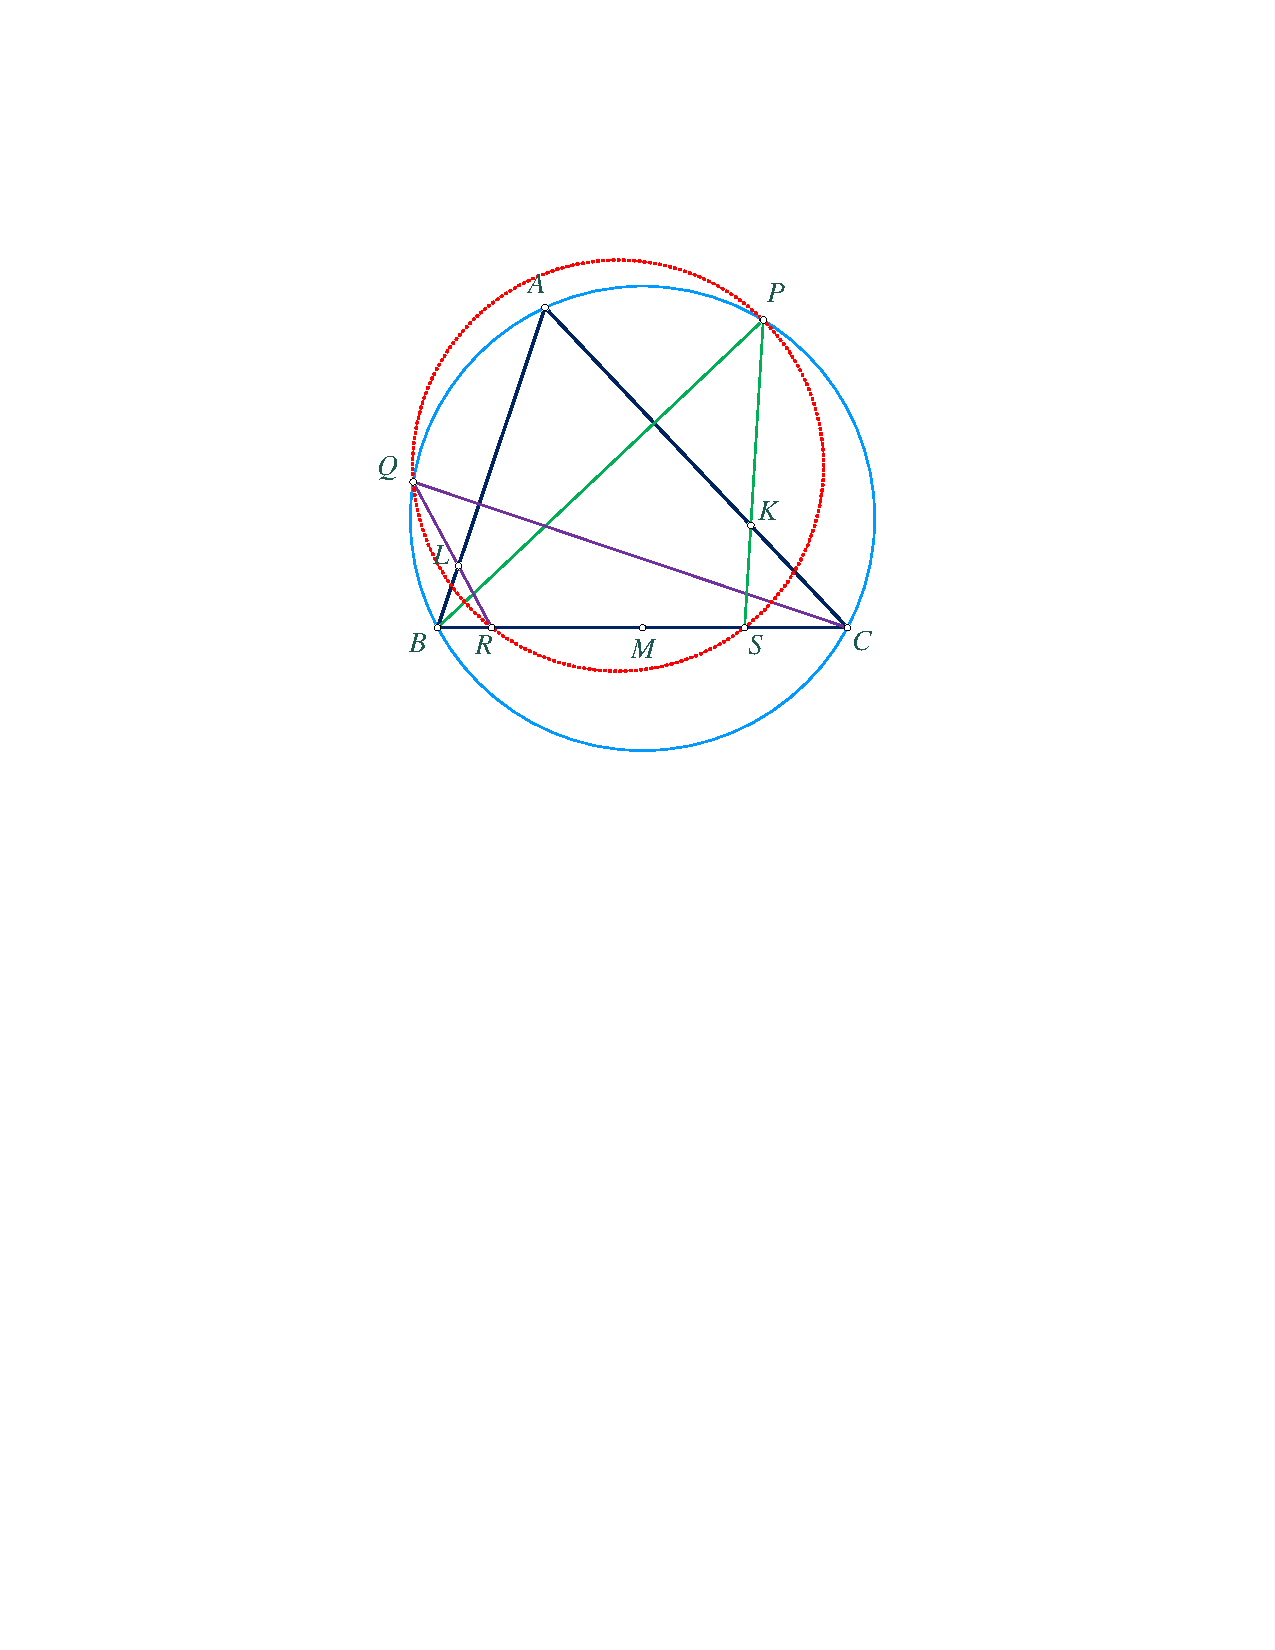
\includegraphics[width=0.82\linewidth]{P624}
		\vspace*{-5pt}
	\end{figure}
	Do tam giác $ABC$ nhọn, nên $P$ thuộc cung $AC$ không chứa $B$, và $Q$ thuộc cung $AB$ không chứa $C$, của $(O)$. Do đó, $A$, $P$, $Q$ nằm cùng phía đối với đường thẳng $BC$. \hfill ($1$)
	\vskip 0.05cm
	Gọi $E$ và $F$ tương ứng là chân đường cao kẻ từ $B$ và $C$ của tam giác $ABC$.
	\vskip 0.05cm
	Vì cùng vuông góc với $AC$ nên $MK \parallel BE$, và vì cùng vuông góc với $AB$ nên $ML \parallel BF$. Mà $M$ là trung điểm của $BC$ (giả thiết), nên suy ra, $K$, $L$ tương ứng là trung điểm của \linebreak$CE$, $BF$. \hfill ($2$)
	\vskip 0.05cm
	Từ ($1$) và ($2$) suy ra, các điểm $R$, $S$ nằm giữa $B$ và $C$. \hfill ($3$)
	\vskip 0.05cm
	Do ($1$) nên từ việc xét đường tròn $(O)$, ta có:
	\begin{align*}
		\angle BQF \!=\! \angle BQC \!=\! \angle BAC \!=\! \angle BPC\! =\! \angle CPE.
	\end{align*}
	Vì thế, tam giác vuông $BFQ$ đồng dạng với tam giác vuông $CEP$. Kết hợp với ($2$), suy ra
	\begin{align*}
		\frac{{FQ}}{{EP}} = \frac{{FB}}{{EC}} = \frac{{FL}}{{EK}}.
	\end{align*}
	Do đó, tam giác vuông $LFQ$ đồng dạng với tam giác vuông $KEP$. Suy ra
	\begin{align*}
		\angle CQR = \angle FQL = \angle EPK = \angle BPS. \tag{$4$}
	\end{align*}
	Do $BCPQ$ là tứ giác nội tiếp nên với lưu ý tới ($3$), ta có:
	\begin{align*}
		\angle RCQ = \angle BCQ = \angle BPQ. \tag{$5$}
	\end{align*}
	Từ ($4$) và ($5$), với lưu ý tới ($3$), suy ra
	\begin{align*}
		\angle BRQ &= \angle CQR + \angle RCQ \\
		&= \angle BPS + \angle BPQ = \angle SPQ.
	\end{align*}
	Do đó, $RSPQ$ là tứ giác nội tiếp, hay bốn điểm $P$, $Q$, $R$, $S$ cùng nằm trên một đường tròn.
	\vskip 0.05cm
	Ta có điều phải chứng minh theo yêu cầu đề bài.
	\vskip 0.05cm
	\textbf{\color{thachthuctoanhoc}Bình luận và Nhận xét}
	\vskip 0.05cm
	Tất cả các lời giải Tạp chí nhận được từ bạn đọc đều là lời giải đúng và hoàn chỉnh.
	\vskip 0.05cm
	\hfill \textbf{\color{thachthuctoanhoc}Hạ Vũ Anh}
	\vskip 0.05cm
	{\color{thachthuctoanhoc}{\usefont{T5}{qag}{b}{n} P625.}}
	(Mức $B$) Cho các số thực dương $a,b,c$. Chứng minh rằng
	\begin{align*}
		\left(\dfrac b{a+c}\right)^2+\left(\dfrac{c}{a+b}\right)^2\ge \dfrac{b^2-bc+c^2}{a^2+bc}.
	\end{align*}
	\textbf{\color{thachthuctoanhoc}Lời giải} (\textit{của người chấm bài})\textbf{\color{thachthuctoanhoc}.}
	\vskip 0.05cm
	Do $a, b, c > 0$ nên theo bất đẳng thức Cauchy -- Schwarz, ta có:
	\begin{align*}
		{\left( {a + c} \right)^2} &= {\left( {a \cdot 1 + \sqrt {bc}  \cdot \frac{{\sqrt c }}{{\sqrt b }}} \right)^2} \\
		&\le \left( {{a^2} + bc} \right)\left( {\frac{c}{b} + 1} \right) \\
		&= \frac{{\left( {{a^2} + bc} \right)\left( {b + c} \right)}}{b}.
	\end{align*}
	Suy ra
	\begin{align*}
		\frac{{{b^2}}}{{{{\left( {a + c} \right)}^2}}} \ge \frac{{{b^3}}}{{\left( {{a^2} + bc} \right)\left( {b + c} \right)}}. \tag{$1$}
	\end{align*}
	Bằng cách hoàn toàn tương tự, ta cũng chứng minh được:
	\begin{align*}
		\frac{{{c^2}}}{{{{\left( {a + b} \right)}^2}}} \ge \frac{{{c^3}}}{{\left( {{a^2} + bc} \right)\left( {b + c} \right)}}. \tag{$2$}
	\end{align*}
	Cộng ($1$) với ($2$), vế theo vế, ta được:
	\begin{align*}
		&{\left( {\frac{b}{{a + c}}} \right)^2} + {\left( {\frac{c}{{a + b}}} \right)^2} \\
		\ge &\frac{{{b^3} + {c^3}}}{{\left( {{a^2} + bc} \right)\left( {b + c} \right)}} = \frac{{{b^2} - bc + {c^2}}}{{{a^2} + bc}}.
	\end{align*}
	Bất đẳng thức của đề bài được chứng minh.
	\vskip 0.05cm
	\textbf{\color{thachthuctoanhoc}Bình luận và Nhận xét}
	\vskip 0.05cm
	$\pmb{1.}$ Dễ thấy, dấu đẳng thức ở bất đẳng thức của đề bài xảy ra khi và chỉ khi $a = b = c$.
	\vskip 0.05cm
	$\pmb{2.}$ Bằng phương pháp của lời giải trên, ta có thể chứng minh được kết quả sau:
	\vskip 0.05cm
	``\textit{Với a, b, c là các số thực dương, ta có:}
	\vskip 0.05cm
	$i)$  $\dfrac{1}{{{{\left( {a + b} \right)}^2}}} + \dfrac{1}{{{{\left( {a + c} \right)}^2}}} \ge \dfrac{1}{{{a^2} + bc}}$;
	\vskip 0.05cm
	$ii)$  $\dfrac{1}{{a + b}} + \dfrac{1}{{b + c}} + \dfrac{1}{{c + a}} \ge \dfrac{a}{{{a^2} + bc}} + \dfrac{b}{{{b^2} + ca}} + \dfrac{c}{{{c^2} + ab}}.$"
	\vskip 0.05cm
	$\pmb{3.}$ Sử dụng bất đẳng thức $i)$ trên đây, ta có thể giải được bài toán bất đẳng thức trong Đề thi chọn đội tuyển Trung Quốc dự thi $IMO$ năm $2004$. Bài toán đó như sau:
	\vskip 0.05cm
	``\textit{Cho các số thực dương $x$, $y$, $z$, $t$ thỏa mãn $xyzt = 1$. Chứng minh rằng}
	\begin{align*}
		\frac{1}{{{{\left( {x \!+\! 1} \!\right)}^2}}} \!+\! \frac{1}{{{{\left( {y \!+\! 1} \!\right)}^2}}} \!+\! \frac{1}{{{{\left( {z \!+\! 1}\! \right)}^2}}} \!+\! \frac{1}{{{{\left( {t \!+\! 1}\! \right)}^2}}} \!\ge\! 1. \text{\color{black}"}
	\end{align*}
	$\pmb{4.}$ Số lời giải Tạp chí nhận được từ bạn đọc không nhiều. Trong số này, rất tiếc, chỉ có hai lời giải đúng; các lời giải còn lại bị sai do người giải bài đã mắc một trong các lỗi cơ bản dưới đây:
	\vskip 0.05cm
	-- Áp dụng phép chuẩn hóa cho bất đẳng thức không thuần nhất;
	\vskip 0.05cm
	-- Từ $0 < x \le y$ suy ra  $\dfrac{1}{x} \le \dfrac{1}{y}$.
	\vskip 0.05cm 
	\hfill \textbf{\color{thachthuctoanhoc}Võ Quốc Bá Cẩn}
	\vskip 0.05cm
	{\color{thachthuctoanhoc}{\usefont{T5}{qag}{b}{n} P626.}}
	(Mức $B$) Xét các tam giác vuông mà độ dài các cạnh là các số nguyên dương và một trong các cạnh góc vuông có độ dài là $2021^{22}$. Hỏi có bao nhiêu tam giác như vậy? 
	\vskip 0.05cm
	\textbf{\color{thachthuctoanhoc}Lời giải} (\textit{của người chấm bài})\textbf{\color{thachthuctoanhoc}.}
	\vskip 0.05cm
	Trong phần trình bày dưới đây, $|X|$ ký hiệu số phần tử của tập hữu hạn $X$.
	\vskip 0.05cm
	Ký hiệu $x$ là độ dài cạnh huyền và $y$ là độ dài cạnh góc vuông còn lại của tam giác vuông thỏa mãn điều kiện đề bài. Khi đó, $x$, $y$ là các số nguyên dương, $x > y$, và
	\begin{align*}
		{\left( {{{2021}^{22}}} \right)^2} + {y^2} = {x^2}. \tag{$1$}
	\end{align*}
	Hiển nhiên, số tam giác thỏa mãn điều kiện đề bài chính bằng số cặp số nguyên dương $(x, y)$ thỏa mãn $x > y$ và ($1$). \hfill ($2$)
	\vskip 0.05cm
	Ta có
	\begin{align*}
		(1) \Leftrightarrow \left( {x - y} \right)\left( {x + y} \right) = {2021^{44}}. \tag{$3$}
	\end{align*}
	Do đó, số cặp số nguyên dương $(x, y)$ thỏa mãn $x > y$ và ($1$) bằng số cặp số nguyên dương $(x, y)$ thỏa mãn $x > y$ và ($3$). \hfill ($4$)
	\vskip 0.05cm
	Dưới đây, ta sẽ gọi cặp số nguyên dương thỏa mãn các điều kiện vừa nêu trên là \textit{cặp số thuận}.
	\vskip 0.05cm
	Xét một cặp số thuận tùy ý. Vì $x > y > 0$ nên  $0 < x - y < x + y$. Do đó
	\begin{align*}
		\left( {x - y} \right)\left( {x + y} \right) > {\left( {x - y} \right)^2};
	\end{align*}
	kết hợp với ($3$), suy ra $x - y < 2021^{22}$. Vì thế, từ ($3$) ta có $x - y$ là một ước dương nhỏ hơn $2021^{22}$  của $2021^{44}$. Do đó, phép đặt ứng
	\begin{align*}
		\text{``cặp số thuận } (x, y) \mapsto   d = x - y\text{"}
	\end{align*}
	sẽ xác lập một ánh xạ, gọi là $f$, từ tập $T$ gồm tất cả các cặp số thuận đến tập $S$ gồm tất cả các ước dương nhỏ hơn $2021^{22}$  của $2021^{44}$.
	\vskip 0.05cm 
	Với $\left( {{x_1},{y_1}} \right),\left( {{x_2},{y_2}} \right)$  tùy ý thuộc $T$, và $\left( {{x_1},{y_1}} \right) \ne \left( {{x_2},{y_2}} \right)$, dễ thấy, ta có ${x_1} - {y_1} \ne {x_2} - {y_2}$  (vì nếu ngược lại,  ${x_1} - {y_1} = {x_2} - {y_2}$, thì theo ($3$), sẽ có  ${x_1} + {y_1} = {x_2} + {y_2}$; dẫn đến $x_1 = x_2$  và  $y_1 = y_2$, mâu thuẫn với giả thiết  $\left( {{x_1},{y_1}} \right) \ne \left( {{x_2},{y_2}} \right)$). Do đó,  $f$ là một đơn ánh từ $T$ đến $S$. \hfill  ($5$)
	\vskip 0.05cm
	Với $d$ tùy ý thuộc $S$, xét cặp số $(x, y)$, xác định bởi:
	\begin{align*}
		x \!=\! \frac{1}{2}\!\!\left(\!\! {d \!+\! \frac{{{{2021}^{44}}}}{d}} \!\!\right) \text{\color{black} và } y \!=\! \frac{1}{2}\!\!\left(\!\! {\frac{{{{2021}^{44}}}}{d} \!-\! d}\!\! \right)
	\end{align*}
	Ta có
	\begin{align*}
		\left( {x \!-\! y} \right)\!\left( {x \!+\! y} \right) \!=\! d \!\cdot\! \frac{{{{2021}^{44}}}}{d} \!=\! {2021^{44}}. \tag{$6$}
	\end{align*}
	Vì $d \in S$ và $2021^{44}$  là một số lẻ nên $x, y \in \mathbb{N^*}$,  và $x > y$. Từ đây và ($6$), suy ra $(x, y) \in T$.
	\vskip 0.05cm
	Do $x - y = d$ nên $d$ là ảnh của $(x, y)$ qua  $f$. Vì thế,  $f$ là một toàn ánh từ $T$ đến $S$. \hfill ($7$)
	\vskip 0.05cm
	Từ ($6$) và ($7$) suy ra,  $f$ là một song ánh từ $T$ đến $S$. Do đó, $|T| = |S|$.
	\vskip 0.05cm 
	Vì ứng với mỗi ước dương nhỏ hơn $2021^{22}$  của $2021^{44}$  có đúng một ước dương lớn hơn $2021^{22}$  của  $2021^{44}$, ứng với mỗi ước dương lớn hơn $2021^{22}$   của  $2021^{44}$ có đúng một ước dương nhỏ hơn $2021^{22}$  của  $2021^{44}$, và $2021^{22}$  là một ước dương của  $2021^{44}$, nên
	\begin{align*}
		|S| = \frac{{N - 1}}{2},
	\end{align*}
	trong đó, $N$ là số ước dương của $2021^{44}$.
	\vskip 0.05cm
	Vì ${2021^{44}} = {43^{44}} \cdot {47^{44}}$ là phân tích chuẩn của $2021^{44}$, nên
	\begin{align*}
		N = \left( {44 + 1} \right)\left( {44 + 1} \right) = 2025.
	\end{align*}
	Do đó
	\begin{align*}
		|S| = \frac{{2025 - 1}}{2} = 1012.
	\end{align*}
	Vì vậy,  $|T| = 1012$. Từ đây và ($4$), ($2$), ta có số tam giác cần tìm theo yêu cầu đề bài là $1012$.
	\vskip 0.05cm
	\textbf{\color{thachthuctoanhoc}Bình luận và Nhận xét}
	\vskip 0.05cm
	$\pmb{1.}$ Lập luận ``Từ $x - y$ là một ước dương nhỏ hơn $2021^{22}$  của  $2021^{44}$, và với mỗi ước dương nhỏ hơn $2021^{22}$  của $2021^{44}$  xác định được ít nhất một cặp số thuận (theo ``định nghĩa" trong lời giải trên), suy ra, số cặp số thuận bằng số ước dương nhỏ hơn $2021^{22}$  của  $2021^{44}$" là một lập luận sai kiến thức cơ bản; vì lập luận đó tương đương với khẳng định ``nếu tồn tại một toàn ánh từ tập $X$ đến tập $Y$ thì  $|X| = |Y|$".
	\vskip 0.05cm
	$\pmb{2.}$ Trong số các lời giải Tạp chí đã nhận được từ bạn đọc, rất tiếc, có một lời giải sai (do người giải bài đếm ``thừa", vì quên rằng $20216{22}$  là một ước dương của  $2021^{44}$) và một lời giải không hoàn chỉnh (do người giải bài lập luận thiếu chặt chẽ, thiếu chính xác).
	\vskip 0.05cm
	\hfill \textbf{\color{thachthuctoanhoc}Hà Thanh}
	\vskip 0.05cm
	{\color{thachthuctoanhoc}{\usefont{T5}{qag}{b}{n} P627.}}
	(Mức $A$) Xét $x,y$ là hai số thực dương thoả mãn $xy\ge 1$. Tìm giá trị lớn nhất của biểu thức
	\begin{align*}
		P=\dfrac1{\sqrt{x^2+1}}+\dfrac1{\sqrt{y^2+1}}-\dfrac3{4(x+y)}.
	\end{align*}
	\textbf{\color{thachthuctoanhoc}Lời giải} (\textit{dựa theo lời giải của bạn Trần Minh Hoàng, lớp $10$T$1$, trường THPT chuyên Hà Tĩnh, tỉnh Hà Tĩnh})\textbf{\color{thachthuctoanhoc}.}
	\vskip 0.05cm
	Đặt $a = \frac{1}{{\sqrt {{x^2} + 1} }}$  và  $b = \frac{1}{{\sqrt {{y^2} + 1} }}$; ta có $a, b > 0$, và $P$ được viết lại dưới dạng:
	\begin{align*}
		P = a + b - \frac{3}{{4\left( {x + y} \right)}}. \tag{$1$}
	\end{align*}
	Áp dụng bất đẳng thức Cauchy -- Schwarz cho hai bộ số thực $(x, 1)$ và $(1, y)$, ta được:
	\begin{align*}
		{\left( {x + y} \right)^2} \le \left( {{x^2} + 1} \right)\left( {{y^2} + 1} \right);
	\end{align*}
	suy ra
	\begin{align*}
		\frac{1}{{x + y}} &\ge \frac{1}{{\sqrt {\left( {{x^2} + 1} \right)\left( {{y^2} + 1} \right)} }} \\
		&= ab \quad(\text{\color{black}do } x,y >0) \tag{$2$}
	\end{align*}
	Từ ($1$) và ($2$), ta có
	\begin{align*}
		P \le a + b - \frac{3}{4}ab. \tag{$3$}
	\end{align*}
	Vì $xy \ge 1$ nên
	\begin{align*}
		{a^2} \!+\! {b^2} &= \frac{1}{{{x^2} \!+\! 1}} \!+\! \frac{1}{{{y^2} \!+\! 1}} \!=\! \frac{{{x^2} \!+\! {y^2} \!+\! 2}}{{\left( {{x^2} \!+\! 1} \right)\!\left( {{y^2} \!+\! 1} \right)}} \\
		&= \frac{{{x^2} + {y^2} + 2}}{{{{\left( {x + y} \right)}^2} + {{\left( {xy - 1} \right)}^2}}} \\
		&\le \frac{{{{\left( {x + y} \right)}^2}}}{{{{\left( {x + y} \right)}^2} + {{\left( {xy - 1} \right)}^2}}} \le 1.
	\end{align*}
	Do đó, ${\left( {a + b} \right)^2} \le 2ab + 1$; suy ra
	\begin{align*}
		ab \ge \frac{1}{2}{\left( {a + b} \right)^2} - \frac{1}{2}.
	\end{align*}
	Từ ($3$) và ($4$), ta được:
	\begin{align*}
		P &\le a + b - \frac{3}{8}{\left( {a + b} \right)^2} + \frac{3}{8}\\
		 &= \frac{{25}}{{24}} - {\left( {a + b - \frac{4}{3}} \right)^2} \le \frac{{25}}{{24}}.
	\end{align*}
	Hơn nữa, với  $x = \dfrac{{9 - 4\sqrt 2 }}{7}$ và  $y = \dfrac{{9 + 4\sqrt 2 }}{7}$, ta có $x, y > 0, xy = 1$, và bằng tính toán trực tiếp, dễ dàng tính được  $P = \dfrac{25}{24}$.
	\vskip 0.05cm
	Vì vậy, giá trị lớn nhất của $P$ bằng  $\dfrac{25}{24}$.
	\vskip 0.05cm
	\textbf{\color{thachthuctoanhoc}Bình luận và Nhận xét}
	\vskip 0.05cm
	$\pmb{1.}$ Các giá trị $x, y$ ở phần cuối của Lời giải trên được tìm ra từ việc xét khả năng xảy ra dấu đẳng thức ở các bất đẳng thức trong lời giải.
	\vskip 0.05cm
	$\pmb{2.}$ Rất tiếc, trong số các lời giải Tạp chí nhận được từ bạn đọc, có một lời giải sai, do người giải bài đã nhầm lẫn trong các đánh giá.
	\vskip 0.05cm
	\hfill\textbf{\color{thachthuctoanhoc}Lưu Thị Thanh Hà}
	\vskip 0.05cm
	{\color{thachthuctoanhoc}{\usefont{T5}{qag}{b}{n} P628.}}
	(Mức $A$) Cho tam giác không cân $ABC$ ngoại tiếp đường tròn $(I)$. Gọi $A_1$, $B_1$, $C_1$ tương ứng là tiếp điểm của $BC$, $CA$, $AB$ với $(I)$; $A_2$, $B_2$, $C_2$ lần lượt là đối xứng của $A_1$, $B_1$, $C_1$ tương ứng qua các đường thẳng $B_1C_1$, $C_1A_1$ và $A_1B_1$. Các đường thẳng $AA_2$, $BC$ cắt nhau tại $A_3$; $BB_2$ và $CA$ cắt nhau tại $B_3$; $CC_2$ và $AB$ cắt nhau tại $C_3$. Chứng minh rằng, $A_3$, $B_3$, $C_3$ thẳng hàng.
	\vskip 0.05cm
	\textbf{\color{thachthuctoanhoc}Lời giải} (\textit{của người chấm bài})\textbf{\color{thachthuctoanhoc}.}
	\begin{figure}[H]
		\centering
		\vspace*{-10pt}
		\captionsetup{labelformat= empty, justification=centering}
		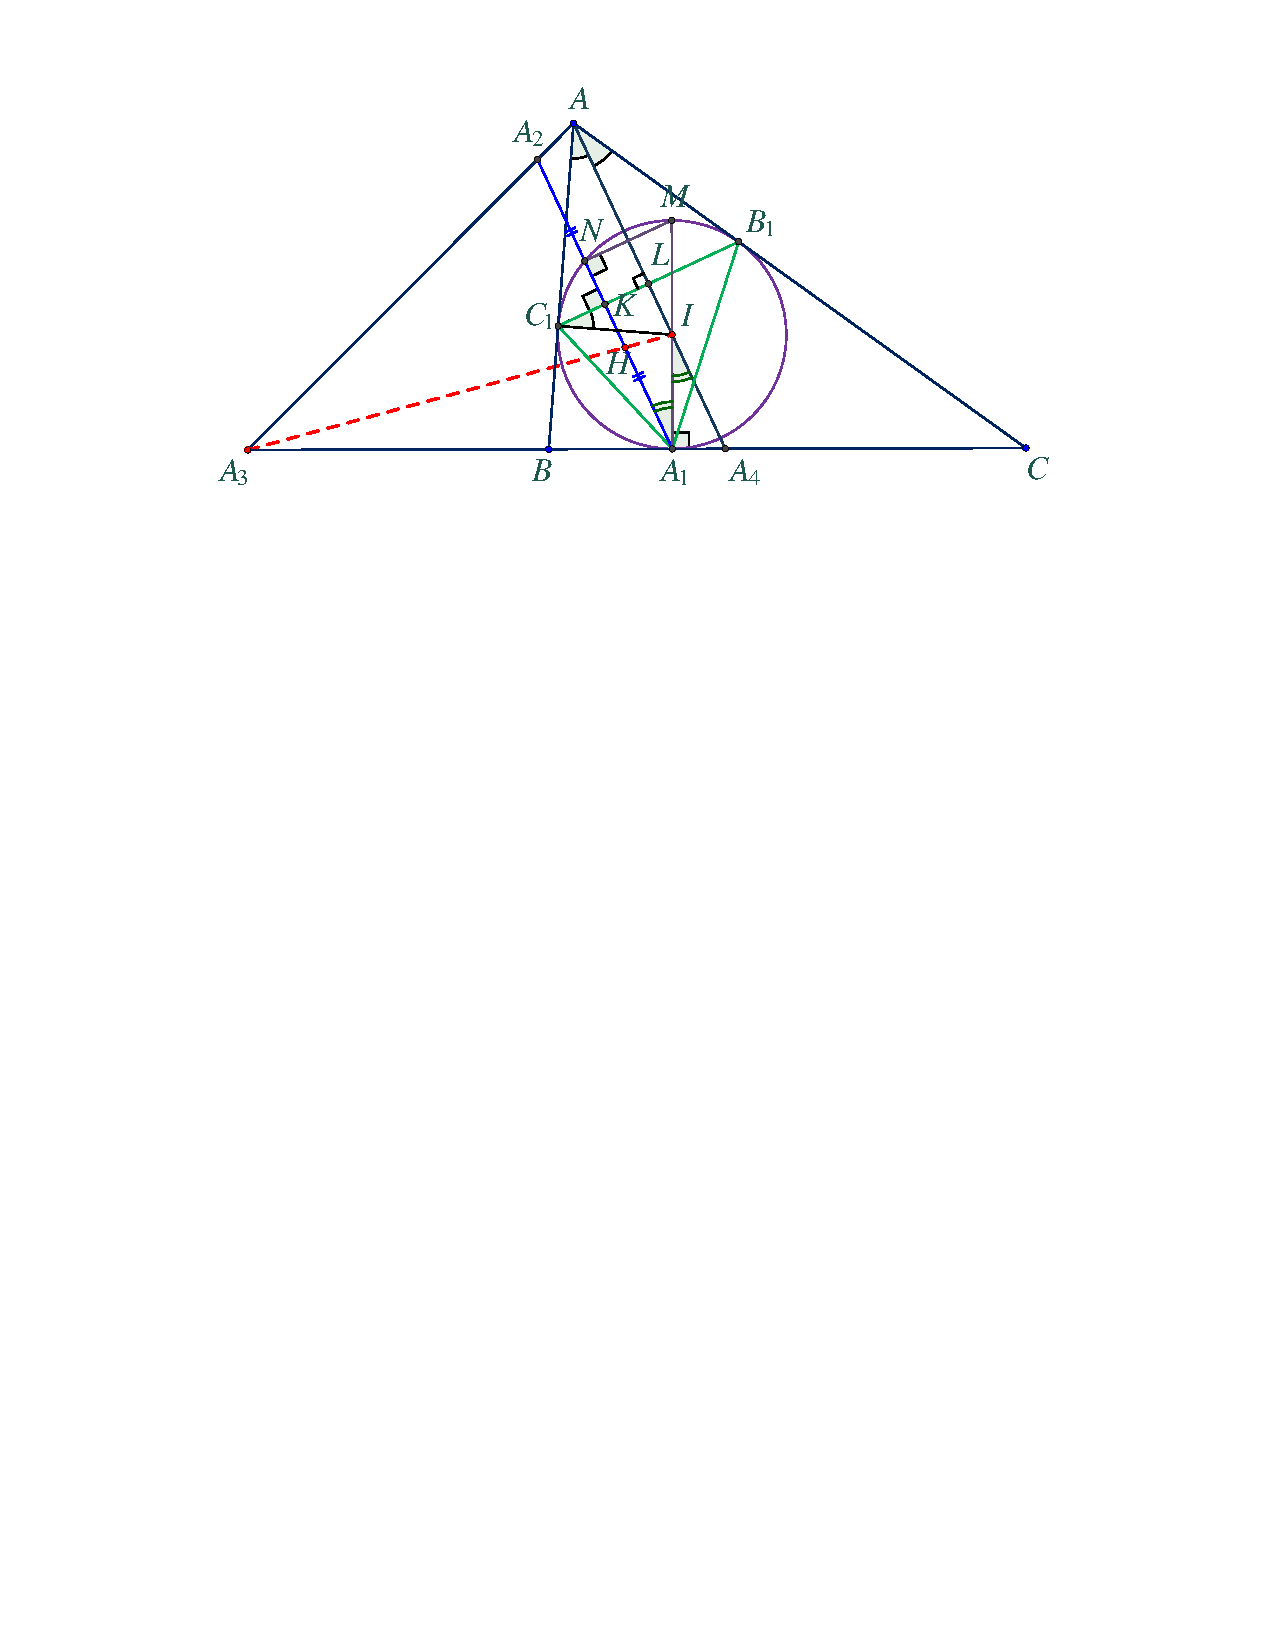
\includegraphics[width=1\linewidth]{P628}
		\vspace*{-15pt}
	\end{figure}
	Gọi $H$ là trực tâm của tam giác $A_1B_1C_1$.
	\vskip 0.05cm 
	Vì tam giác $ABC$ không cân nên nó không là tam giác đều. Suy ra, $A_1B_1C_1$  là tam giác không đều; do đó,  $H \not\equiv I$.
	\vskip 0.05cm
	Do $A_1H \bot B_1C_1$  và  $A_1A_2 \not B_1C_1$, nên $H$ nằm trên đường thẳng  $A_1A_2$.
	\vskip 0.05cm
	Gọi $L$, $A_4$  tương ứng là giao điểm của đường thẳng $AI$ và  $B_1C_1$, $BC$.
	\vskip 0.05cm
	Do tam giác $ABC$ không cân tại $A$, nên $I$ không nằm trên đường thẳng $AA_1$; do đó, $A_4 \not\equiv A_1$    \hfill ($1$)
	\vskip 0.05cm 
	Theo tính chất của hai tiếp tuyến cắt nhau của một đường tròn,  $Ai \bot B_1C_1$; suy ra:
	\vskip 0.05cm
	-- $L$ là trung điểm của $B_1C_1$, \hfill ($2$)
	\vskip 0.05cm
	-- $A_1A_2 \parallel A_4A$  (do cùng vuông góc với  $B_1C_1$ và ($1$)). \hfill($3$)
	\vskip 0.05cm
	Từ ($2$), do $H$, $I$ tương ứng là trực tâm, tâm đường tròn ngoại tiếp tam giác  $A_1B_1C_1$, suy ra
	\begin{align*}
		A_1H = 2IL. \tag{$4$}
	\end{align*}
	Do  $IC_1 \bot AB, IA \bot B_1C_2$, và  $\angle IAC_1, \angle IC_1L$ là các góc nhọn, nên $\angle IAC_1 = \angle IC_1L]$. Do đó, tam giác vuông (tại  $C_1$) $AC_1I$   đồng dạng với tam giác vuông (tại $L$) $C_1LI$.  Suy ra
	\begin{align*}
		\frac{{AI}}{{{C_1}I}} = \frac{{{C_1}I}}{{LI}}.\tag{$5$}
	\end{align*}
	Gọi $M$ là điểm đối xứng với $A_1$  qua $I$. Từ ($5$) và ($4$), ta có:
	\begin{align*}
		\frac{{AI}}{{{C_1}I}} = \frac{{{A_1}M}}{{{A_1}H}} \tag{$6$}
	\end{align*}
	Gọi $K$ là giao điểm của $A_1A_2$ và  $B_1C_1$; gọi $N$ là giao điểm thứ hai (khác $A_1$) của  $A_1A_2$ và đường tròn ($I$).
	\vskip 0.05cm
	Do $A_1, A_2$  đối xứng với nhau qua  $B_1C_1$ nên $K$ là trung điểm $A_1A_2$;  mặt khác, do $H$ là trực tâm tam giác $A_1B_1C_1$, và  $HN \bot B_1C_1$, nên $K$ là trung điểm $HN$. Suy ra, $A_1H = A_2N$; do đó, $A_1N = A_2H$. \hfill  ($7$)
	\vskip 0.05cm
	Từ ($3$) suy ra  $\angle MA_1N = \angle A_4IA_1$; do đó, tam giác vuông (tại  $A_1$) $IA_1A_4$ đồng dạng với tam giác vuông (tại $N$) $A_1NM$.  Suy ra
	\begin{align*}
		\frac{{I{A_1}}}{{{A_1}N}} = \frac{{I{A_4}}}{{{A_1}M}}. \tag{$8$}
	\end{align*}
	Nhân ($6$) với ($8$), vế theo vế, ta được
	\begin{align*}
		\frac{{AI}}{{{A_1}N}} = \frac{{I{A_4}}}{{{A_1}H}};
	\end{align*}
	suy ra,  $\frac{{AI}}{{I{A_4}}} = \frac{{{A_1}N}}{{{A_1}H}}$. Kết hợp với ($7$), ta được:
	\begin{align*}
		\frac{{AI}}{{I{A_4}}} = \frac{{{A_2}H}}{{H{A_1}}}.
	\end{align*}
	Từ đây và ($3$), theo định lý Thales, suy ra, ba điểm  $A_3$, $H$, $I$ thẳng hàng; nói một cách khác, $A_3$  nằm trên đường thẳng $HI$.
	\vskip 0.05cm
	Bằng cách hoàn toàn tương tự, ta cũng chứng minh được, các điểm $B_3, C_3$  nằm trên đường thẳng $HI$. Vì thế, ba điểm  $A_3, B_3 ,C_3$  thẳng hàng.
	\vskip 0.05cm
	\textbf{\color{thachthuctoanhoc}Bình luận và Nhận xét}
	\vskip 0.05cm
	$\pmb{1.}$ Với giả thiết tam giác $ABC$ cân, chẳng hạn tại $A$, \textit{nhưng không đều}, ta có  $A_3 \equiv A_4$ và bốn điểm đôi một phân biệt $A$, $H$, $I$, $A_1$  thẳng hàng. Do vậy, trong trường hợp này,  $A_3$ vẫn nằm trên đường thẳng $HI$. Vì thế, từ lời giải trên dễ thấy, khẳng định của bài ra vẫn đúng, khi thay giả thiết ``không cân" bởi giả thiết (``nhẹ nhàng" hơn) ``\textit{không đều}".
	\vskip 0.05cm
	$\pmb{2.}$ Bài đã ra (với việc thay giả thiết ``không cân" bởi giả thiết ``không đều") là một kết quả hay, thú vị về đường thẳng Euler của một tam giác. Kết quả này đã được Lev Emelyanov công bố trong bài báo ``On the Intercepts of the OI -- Line", đăng trên Forum Geometricorum, Vol. $4$, năm $2004$ (trang $81 - 84$).
	Forum Geometricorum là một Tạp chí về Hình học Euclid cổ điển và các lĩnh vực liên quan, được ấn hành bởi Đại học Atlantic Florida. Bạn đọc có thể tìm đọc Tạp chí này online, tại trang web \url{http://forumgeom.fau.edu.}
	\vskip 0.05cm
	$\pmb{3.}$ Tất cả lời giải Tạp chí nhận được, từ bạn đọc, đều là lời giải đúng.
	\vskip 0.05cm
	\hfill	\textbf{\color{thachthuctoanhoc}Hạ Vũ Anh}
	\vskip 0.05cm
	{\color{thachthuctoanhoc}{\usefont{T5}{qag}{b}{n} P629.}}
	(Mức $A$) Cho $n$ là một số nguyên dương có tính chất: không tồn tại các số nguyên dương $a,b,c$ sao cho $\dfrac4n=\dfrac 1a+\dfrac 1b+\dfrac 1c.$ Chứng minh rằng, tồn tại các số nguyên không âm $u,v$ sao cho: $n=u^2+v^2$.  
	\vskip 0.05cm
	\textbf{\color{thachthuctoanhoc}Lời giải} (\textit{phỏng theo lời giải của bạn Hồ Trần Khánh Linh, lớp $12$ Toán $2$, trường THPT chuyên ĐHSP, ĐHSP Hà Nội})\textbf{\color{thachthuctoanhoc}.}
	\vskip 0.05cm
	Trong Lời giải này, ta quy ước gọi một số nguyên dương là \textit{số tốt}, nếu nó biểu diễn được dưới dạng tổng bình phương của hai số nguyên không âm.
	\vskip 0.05cm
	Trước hết, dễ thấy $n = 1$ là một số nguyên dương có tính chất đã nêu trong đề bài, vì $\dfrac{4}{1} = 4$ và với mọi $a, b, c$ nguyên dương,\linebreak $\dfrac{1}{a} + \dfrac{1}{b} + \dfrac{1}{c} \le 3$.
	\vskip 0.05cm
	Do  $1 = 0^2 + 1^2$, nên $n = 1$ là một số tốt. \hfill ($1$)
	\vskip 0.05cm
	Xét $n > 1$.
	\vskip 0.05cm
	Ta có hai Nhận xét sau:
	\vskip 0.05cm
	\textbf{\color{thachthuctoanhoc}Nhận xét} $\pmb{1:}$ \textit{$n$ không thể là số chẵn}, vì nếu ngược lại, $n$ là số chẵn, thì chọn  $a= \dfrac{n}{2}$, \linebreak$b = c = n$, ta sẽ có $a,b,c \in \mathbb{N^*}$  và
	\begin{align*}
		\frac{1}{a} + \frac{1}{b} + \frac{1}{c} 
		= \frac{2}{n} + \frac{1}{n} + \frac{1}{n} = \frac{4}{n}.
	\end{align*}
	\textbf{\color{thachthuctoanhoc}Nhận xét} $\pmb{2:}$ $n$ \textit{không thể có ước nguyên tố dạng} $4k + 3$, $k \in \mathbb{N}$, vì nếu ngược lại, $n$ có ước nguyên tố $p$ có dạng đó, thì chọn  $a = \frac{{n\left( {p + 1} \right)}}{4}$,  $b = c = \frac{{n\left( {p + 1} \right)}}{{2p}}$, ta sẽ có $a,b,c \in \mathbb{N^*}$  và
	\begin{align*}
		&\frac{1}{a} + \frac{1}{b} + \frac{1}{c} \\
		= &\frac{4}{{n\left( {p + 1} \right)}} + \frac{{2p}}{{n\left( {p + 1} \right)}} + \frac{{2p}}{{n\left( {p + 1} \right)}} = \frac{4}{n}.
	\end{align*}
	Từ hai Nhận xét trên suy ra, $n$ chỉ có ước nguyên tố dạng $4k + 1$, $k \in \mathbb{N^*}$  \hfill        ($2$)
	\vskip 0.05cm
	Theo định lý Fermat về tổng hai số chính phương, mọi số nguyên tố có dạng $4k + 1$, $k \in \mathbb{N^*}$  đều là số tốt. \hfill ($3$)
	\vskip 0.05cm
	Do
	\begin{align*}
		\left( {{x^2} + {y^2}} \right)\!\!\left( {{s^2} + {t^2}} \right) \!=\! {\left( {xs + yt} \right)^2} \!+\! {\left( {xt - ys} \right)^2},
	\end{align*}
	nên tích của hai số tốt là một số tốt. \hfill ($4$)
	\vskip 0.05cm
	Từ ($2$), ($3$) và ($4$) suy ra, mọi số $n > 1$ đều là số tốt. ($5$)
	\vskip 0.05cm
	Từ ($1$) và ($5$) hiển nhiên có: mọi số $n$ được cho ở đề bài đều là số tốt; nghĩa là, tồn tại các số nguyên không âm $u$, $v$ sao cho $n = u^2 + v^2$.
	\vskip 0.05cm 
	\textbf{\color{thachthuctoanhoc}Bình luận và Nhận xét}
	\vskip 0.05cm
	$\pmb{1.}$ Lời giải trên cho thấy, bài đã ra là một khai thác nhẹ nhàng, thú vị từ định lý Fermat về tổng của hai số chính phương.
	\vskip 0.05cm
	$\pmb{2.}$ Để tiện cho việc theo dõi của bạn đọc, xin nhắc lại định lý vừa nêu trên.
	\vskip 0.05cm
	\textbf{\color{thachthuctoanhoc}Định lý Fermat về tổng của hai số chính phương.} \textit{Số nguyên tố lẻ p biểu diễn được dưới dạng tổng của hai số chính phương khi và chỉ khi $p \equiv 1\left( {\bmod 4} \right)$.}
	\vskip 0.05cm 
	Vì một số chính phương chỉ có số dư là $0$ hoặc $1$ trong phép chia cho $4$, nên điều kiện cần (chỉ khi) nêu trong định lý trên là hiển nhiên.
	\vskip 0.05cm
	Đối với điều kiện đủ (khi), có nhiều cách để chứng minh; một trong các cách đó, là chứng minh theo lược đồ sau (được Euler đưa ra vào năm $1747$):
	\vskip 0.05cm
	-- Quy ước gọi một số nguyên dương là \textit{số tốt}, nếu nó biểu diễn được dưới dạng tổng của hai số chính phương.
	\vskip 0.05cm
	-- Bằng phương pháp phản chứng, chứng minh bổ đề sau:
	\vskip 0.05cm
	\textbf{\color{thachthuctoanhoc}Bổ đề.} \textit{Nếu $a$, $b$ là hai số nguyên dương, nguyên tố cùng nhau, thì mọi ước dương lớn hơn $1$ của $a^2 + b^2$  đều là số tốt.}
	\vskip 0.05cm
	-- Xét số nguyên tố $p$ tùy ý có dạng $p = 4k + 1$, $k \in \mathbb{N^*}$.
	\vskip 0.05cm  
	Theo định lý nhỏ Fermat, với mọi $m \in \{1, 2, \ldots, 4k\}$, ${m^{4k}} \equiv 1\left( {\bmod p} \right)$.
	\vskip 0.05cm
	Do đó, với mỗi $m \in \{2, \ldots, 4k\}$, ta có:
	\begin{align*}
		&{m^{4k}} - {\left( {m - 1} \right)^{4k}} \\
		= &\left( {{m^{2k}} - {{\left( {m - 1} \right)}^{2k}}} \right)\left( {{m^{2k}} + {{\left( {m - 1} \right)}^{2k}}} \right) \\
		&\equiv 0\left( {\bmod p} \right).
	\end{align*}
	Từ đó, do $p$ là số nguyên tố, suy ra
	\begin{align*}
		&\left. {p} \right|\left( {{m^{2k}} - {{\left( {m - 1} \right)}^{2k}}} \right),\\
		 \text{\color{black} hoặc } &\left. {p} \right|\left( {{m^{2k}} + {{\left( {m - 1} \right)}^{2k}}} \right).
	\end{align*}
	Dễ thấy, không thể xảy ra trường hợp
	\begin{align*}
		\left. {p} \right|\left( {{m^{2k}} - {{\left( {m - 1} \right)}^{2k}}} \right)
	\end{align*}
	với mọi $m \in \{2, \ldots, 4k\}$, vì nếu như thế thì phương trình
	\begin{align*}
		{x^{2k}} - 1 \equiv 0\left( {\bmod p} \right)
	\end{align*}
	sẽ có $4k$ nghiệm (là $1, 2, \ldots, 4k$), trái với định lý Lagrange.
	\vskip 0.05cm
	Vì vậy, tồn tại $m \in \{2, \ldots, 4k\}$, sao cho
	\begin{align*}
		\left. {p} \right|\left( {{m^{2k}} + {{\left( {m - 1} \right)}^{2k}}} \right).
	\end{align*}
	Từ đó, do $(m, m - 1) = 1$ nên theo Bổ đề trên, $p$ là một số tốt; nghĩa là, $p$ biểu diễn được dưới dạng tổng của hai số chính phương.
	\vskip 0.05cm
	(Về định lý Lagrange, bạn đọc có thể tham khảo trong Tạp chí Pi, số $10$ năm $2022$, trang … .)
	\vskip 0.05cm
	$\pmb{3.}$ Một số kết quả thú vị, có liên quan gần với định lý Fermat:
	\vskip 0.05cm
	\textit{Với $p$ là một số nguyên tố, ta có:}
	\vskip 0.05cm
	$\diamond$ $p = {x^2} + 2{y^2} \Leftrightarrow p \equiv 1,3\left( {\bmod 8} \right)$;
	\vskip 0.05cm
	$\diamond$ $p = {x^2} + 3{y^2} \Leftrightarrow p \equiv 1\left( {\bmod 3} \right)$;
	\vskip 0.05cm
	$\diamond$ $p = {x^2} + 5{y^2} \Leftrightarrow p \equiv 1,9\left( {\bmod 20} \right)$;
	\vskip 0.05cm
	$\diamond$ $2p = {x^2} + 5{y^2} \Leftrightarrow p \equiv 3,7\left( {\bmod 20} \right)$.
	\vskip 0.05cm
	(Trong các kết quả trên, $x$, $y$ là các số tự nhiên.)
	\vskip 0.05cm
	Các kết quả $1$, $2$ (theo thứ tự liệt kê) do Fermat tìm ra; các kết quả $3$, $4$ do Euler dự đoán, và sau đó, được Lagrange chứng minh.
	\vskip 0.05cm
	$\pmb{4.}$ Nếu bỏ qua các lỗi ``chính tả" thì trong số các lời giải Tạp chí đã nhận được từ bạn đọc, chỉ có lời giải của bạn \textit{Hồ Trần Khánh Linh} được coi là hoàn chỉnh. Tất cả các lời giải còn lại hoặc không hoàn chỉnh (do người giải bài thiếu xét trường hợp $n = 1$), hoặc sai (do người giải bài ngộ nhận rằng một số nguyên tố chỉ hoặc có dạng $4k + 1$, $k \in \mathbb{N^*}$, hoặc có dạng $4k + 3, k\in \mathbb{N}$).
	\vskip 0.05cm
	\hfill \textbf{\color{thachthuctoanhoc}Lưu Thị Thanh Hà}
	\vskip 0.05cm
	{\color{thachthuctoanhoc}{\usefont{T5}{qag}{b}{n} P630.}}
	(Mức $A$) Bạn Pi ghi lên bảng một số $1$; sau đó, thực hiện việc xoá và ghi thêm số, theo quy tắc:  Mỗi lần, xoá một số $N$ tuỳ ý đang có trên bảng, rồi ghi thêm lên bảng số $N+1$,  hoặc số $3N$.
	\vskip 0.05cm
	Pi thực hiện việc xoá và ghi thêm số, để trên bảng có một số chia hết cho $47$, và Pi dừng việc xoá--ghi thêm số ngay sau khi ghi được một số như vậy. 
	\vskip 0.05cm
	Mỗi lần xoá số $N$ và ghi số $3N$, Pi được nhận một viên kẹo xốp, còn nếu ghi số $N+1$ thì được nhận một viên kẹo dẻo. Vì không thích kẹo dẻo, nên trong quá trình xoá-ghi thêm số, Pi luôn cố gắng để được nhận kẹo xốp. Hỏi, Pi phải nhận ít nhất bao nhiêu viên kẹo dẻo? 
	\vskip 0.05cm
	\textbf{\color{thachthuctoanhoc}Lời giải} (\textit{dựa theo lời giải của bạn Trần Minh Hoàng, lớp $10$T$1$, trường THPT chuyên Hà Tĩnh, tỉnh Hà Tĩnh}).
	\vskip 0.05cm
	Gọi mỗi lần xóa số $N$ và ghi số $3N$ là một ``\textit{bước nhân}", mỗi lần lần xóa số $N$ và ghi số $N + 1$ là một ``\textit{bước cộng}".
	\vskip 0.05cm
	Mỗi quá trình thực hiện việc xóa và ghi thêm số, kể từ lúc bắt đầu thực hiện đến khi dừng lại, được gọi tắt là một \textit{quá trình}.
	\vskip 0.05cm
	Do ban đầu, ở trên bảng chỉ có một số, nên từ quy tắc xóa và ghi số suy ra, tại mọi thời điểm, ở trên bảng chỉ có đúng một số.            \hfill ($1$)
	\vskip 0.05cm
	Tiếp theo, nhận thấy, $47|3N$  khi và chỉ khi $47|N$  (do $(3, 47) = 1$). Do đó, bước cuối cùng của mọi quá trình đều phải là một bước cộng. \hfill ($2$)
	\vskip 0.05cm
	Vì vậy, gọi $k$ là số bước cộng của một quá trình tùy ý, ta có $k \ge 1$.\hfill ($3$)
	\vskip 0.05cm
	Giả sử tồn tại một quá trình có $k = 1$, và giả sử quá trình này gồm $m + 1$ bước ($m \in \mathbb{N^*}$).
	\vskip 0.05cm
	Khi đó, theo ($1$) và ($2$), số được ghi lên bảng ở bước cuối cùng của quá trình là $3^m + 1$. Vì thế
	\begin{align*}
		47|{3^m} + 1; \tag{$4$}
	\end{align*}
	suy ra,  $47|{3^{2m}} - 1$. Do đó, ký hiệu $h$ là cấp của $3$ modulo $7$, ta có  $h|2m$. \hfill   ($5$)
	\vskip 0.05cm
	Vì
	\begin{align*}
		{3^{23}} = {\left( {{3^5}} \right)^4} \cdot {3^3} &\equiv {8^4} \cdot 27 \equiv {17^2} \cdot 27 \\
		&\equiv 7 \cdot 27 \equiv 1\left( {\bmod 47} \right),
	\end{align*}
	nên $h|23$.  Mà $23$ là số nguyên tố, và ${3^1}\not  \equiv 1\left( {\bmod 47} \right)$,  nên $h = 23$. Vì thế, theo ($5$),  $23|2m$; do đó, $23|m$  (vì $(2, 23) = 1$). Suy ra, $47|3^m-1$; kết hợp với ($4$), ta được
	\begin{align*}
		2 = \left( {{3^m} + 1} \right) - \left( {{3^m} - 1} \right) \equiv 0\left( {\bmod 47} \right),
	\end{align*}
	là điều vô lý.
	\vskip 0.05cm
	Vì vậy, không tồn tại quá trình nào có $k = 1$. Do đó, từ ($3$) suy ra, $k \ge 2$.\hfill      ($6$)
	\vskip 0.05cm
	Xét việc thực hiện phép xóa và ghi thêm số, như sau:
	\vskip 0.05cm
	-- Bảy lần đầu tiên: thực hiện bước nhân;
	\vskip 0.05cm
	-- Lần thứ $8$: thực hiện bước cộng;
	\vskip 0.05cm
	-- Hai lần tiếp theo: thực hiện bước nhân;
	\vskip 0.05cm
	-- Lần thứ $11$: thực hiện bước cộng.
	\vskip 0.05cm
	Do $1\not  \equiv 0\left( {\bmod 47} \right)$  và $(3, 47) = 1$, nên tất cả các số được ghi lên bảng ở bảy lần đầu tiên đều không chia hết cho $47$.
	\vskip 0.05cm
	Số được ghi ở lần thứ $8$ là  ${3^7} + 1\not  \equiv 0\left( {\bmod 47} \right)$, nên các số được ghi ở hai lần tiếp theo cũng không chia hết cho $47$.
	\vskip 0.05cm
	Số được ghi ở lần thứ $11$ là  $\left( {{3^7} + 1} \right) \cdot {3^2} + 1 \equiv 26 \cdot 9 + 1 \equiv 0\left( {\bmod 47} \right)$.
	\vskip 0.05cm
	Vì vậy, việc thực hiện phép xóa và ghi thêm số như trên cho ta một quá trình, với số bước cộng bằng $2$. Điều này và ($6$) cho thấy, giá trị nhỏ nhất của $k$ bằng $2$. Nói một cách khác, Pi phải nhận ít nhất $2$ viên kẹo dẻo.
	\vskip 0.05cm
	\textbf{\color{thachthuctoanhoc}Bình luận và Nhận xét}
	\vskip 0.05cm
	Tất cả lời giải Tạp chí đã nhận được, từ bạn đọc, đều là lời giải đúng.
	\vskip 0.05cm
	\hfill\textbf{\color{thachthuctoanhoc}Nguyễn Khắc Minh}
\end{multicols}
\begin{center}
	\textbf{\color{thachthuctoanhoc}DANH SÁCH HỌC SINH CÓ LỜI GIẢI HOÀN CHỈNH}
\end{center}
\textit{Trong các ngoặc đơn ở phần dưới đây, sau tên lớp là mã hiệu của các bài toán mà học sinh có lời giải hoàn chỉnh.}
\begin{multicols}{2}
	\textbf{\color{thachthuctoanhoc}KHỐI THCS}
	\vskip 0.05cm
	$\bullet$ Trường \textbf{\color{thachthuctoanhoc}THCS Long Bình Điền}, Tỉnh Tiền Giang: \textit{Võ Trần Tiến} (lớp $8^5$,  P$621$).
	\vskip 0.05cm
	\textbf{\color{thachthuctoanhoc}KHỐI THPT}
	\vskip 0.05cm
	$\bullet$ Trường \textbf{\color{thachthuctoanhoc}THPT số $\pmb{2}$ Phù Cát}, Tỉnh Bình Định: \textit{Nguyễn Hữu Trí} (lớp $10$A$1$; P$624$).
	\vskip 0.05cm
	$\bullet$ Trường \textbf{\color{thachthuctoanhoc}THPT chuyên Lê Quý Đôn}, Tp. Đà Nẵng: \textit{Nguyễn Châu Tuấn Kiệt} (lớp $10$A$2$; P$624$, P$625$, P$628$).
	\vskip 0.05cm
	$\bullet$ Trường \textbf{\color{thachthuctoanhoc}THPT chuyên Nguyễn Quang Diêu}, Tỉnh Đồng Tháp: \textit{Lâm Nhật Tiến} (lớp $10$T$1$; P$624$).
	\vskip 0.05cm
	$\bullet$ Trường \textbf{\color{thachthuctoanhoc}THPT chuyên Hà Tĩnh}, Tỉnh Hà Tĩnh: \textit{Trần Minh Hoàng} (lớp $10$T$1$; P$627$, P$628$, P$630$).
	\vskip 0.05cm
	$\bullet$ Trường \textbf{\color{thachthuctoanhoc}THPT Gia Định}, Tp. Hồ Chí Minh: \textit{Lê Nam Khánh} (lớp $11$CT; P$624$, P$628$), \textit{Nguyễn Hà Ngọc Uyên} (lớp $12$CT; P$624$).
	\vskip 0.05cm
	$\bullet$ Trường \textbf{\color{thachthuctoanhoc}THPT chuyên Hưng Yên}, Tỉnh Hưng Yên: \textit{Trần Hữu Dương} (lớp $11$ Toán $1$; P$621$, P$625$).
	\vskip 0.05cm
	$\bullet$ Trường \textbf{\color{thachthuctoanhoc}THPT chuyên Lương Văn Chánh}, Tỉnh Phú Yên: \textit{Nguyễn Thị Bảo Tiên} (lớp $11$ Toán $1$; P$624$).
	\vskip 0.05cm
	$\bullet$ Trường \textbf{\color{thachthuctoanhoc}THPT chuyên Khoa học tự nhiên}, ĐH Khoa học tự nhiên -- ĐHQG Hà Nội: \textit{Vương Khánh Toàn} (lớp $10$A$1$ Toán; P$627$).
	\vskip 0.05cm
	$\bullet$ Trường \textbf{\color{thachthuctoanhoc}THPT chuyên Sư phạm}, ĐH Sư phạm Hà Nội: \textit{Hồ Trần Khánh Linh} (lớp $12$ Toán $2$; P$627$, P$628$, P$629$, P$630$).
\end{multicols}

